% ============================================================================
%  DRAFT v0.1  —  for advisor review
%  Build: any standard TeX distribution, or Overleaf; no extra .sty needed.
%  To switch to the ACL template, replace the \documentclass below with
%     \documentclass[11pt]{article}\usepackage[review]{acl}
%  and drop geometry/mathptmx (acl.sty provides its own layout and fonts).
%  NOTE ON THE BIBLIOGRAPHY: every entry in refs.bib has been checked against a
%  fetched authoritative record; see the header comment in that file.
% ============================================================================
\documentclass[11pt]{article}
\usepackage[utf8]{inputenc}
\usepackage[T1]{fontenc}
\usepackage[margin=1in]{geometry}
\usepackage{amsmath,amssymb}
% mathptmx gives Times for text AND math (standard psnfss package). The previous
% \usepackage{times} changed only the text and left math in Computer Modern, mixing two
% typefaces. If this line ever fails to compile, revert to \usepackage{times}: it still
% builds, the math font is just inconsistent.
\usepackage{mathptmx}
\usepackage{graphicx}
\usepackage{booktabs}
\usepackage{multirow}
\usepackage{xcolor}
\usepackage[numbers,sort&compress]{natbib}
\usepackage[hidelinks]{hyperref}
\usepackage{caption}
% 附录里的表刻意做成非浮动（captionof + center），hypcap 对它们无意义，
% 关掉以免日志里出现 9 条 "hypcap=true will be ignored" 噪音、掩盖真问题。
\captionsetup{font=small,labelfont=bf,hypcap=false}
\newcommand{\todo}[1]{\textcolor{red}{[TODO: #1]}}
% \ensuremath：\mask 在正文里是数学模式（$\mask=...$），在表格/图注里是文本模式。
% 不加 \ensuremath 的话，文本模式下的 \mathrm 会触发 "Missing $ inserted"，
% 全文十余处会累积成可恢复错误（曾导致附录尾部内容被吞）。
\newcommand{\mask}{\ensuremath{\mathrm{masking}}}

\title{\textbf{What Apparent Gains Hide:\\ Measuring, Validating, and Localising\\ Parametric-Memory Contamination in RAG Evaluation}}
\author{Anonymous draft v0.1 --- for internal review}
\date{\today}

\begin{document}
\maketitle

\begin{abstract}
Retrieval-augmented generation (RAG) is standardly evaluated by comparing a model
\emph{with} retrieved evidence against the same model \emph{without} it. We show that
this comparison can systematically understate what the evidence actually contributes,
because the no-evidence baseline is inflated by \emph{parametric memory}: the model may
already know the answer. We formalize the problem with a four-arm design over a
controlled-substitution corpus and define the resulting gap as \emph{masking}. On a
single-hop factoid pool (TriviaQA, $n{=}432$) masking reaches \textbf{+0.23} on the
oracle-context line (C-line) and \textbf{+0.31} on the shared-corpus retrieval line
(B-line; the largest value comes from a cross-generation model that is not
modality-matched), and on the B-line it is positive in \textbf{12/12} model$\times k$
configurations
(\textbf{10/12} with 95\% CI excluding zero; both exceptions come from the smallest model,
whose closed-book floor leaves nothing to leak); on the $k{=}1$ axis its point
estimate rises at every step of the model scale, and across the $17$ cells that share the
pool masking grows with the model's closed-book accuracy at a slope of $0.50$ (95\% CI
$0.44$--$0.57$; $0.52$ on the oracle-context line and $0.50$ on the retrieved line, which we
therefore pool)---well below the slope of $1$ that a constant manipulation cost would force,
so the relation is not a restatement of the identity. The $k{=}5$ axis has one reversal,
which we report. We then audit the manipulation
itself: prior work that rewrites a passage to probe parametric memory does not report
whether those rewrites are valid. A human audit of a 20.2\% sample of the \emph{pre-fix}
corpus finds \textbf{24.4\%} of
constructed items invalid; we trace the causes to a numeric boundary bug, an unconstrained
date-borrowing rule, and a construction assumption that a unique literal match locates the
answer, then show in ablations that the conclusions are stable or stronger afterwards.
Finally, we give an exact decomposition, $\mask=(a-c)-(b-d)$. It is an accounting identity
rather than a testable hypothesis, and we do not present it as one: its content is to
identify which term is \emph{movable}. Because the substituted answer
is borrowed from another question, the closed-book arm on that key sits at the floor, so
$(a-c)$ is numerically close to $a$ itself and the only term a change of setting can move is
the manipulation cost $(b-d)$.
That reading implies a
genuine, falsifiable prediction about a stronger model, which we pre-registered and which
\emph{failed}.
On multi-hop questions (HotpotQA,
$n{=}393$), where the model has almost no parametric memory, masking is not merely
undetected but bounded: an equivalence test excludes effects larger than five accuracy
points for all five models. The boundary is not specific to multi-hop questions: on
\emph{entity}-type answers, where we construct a borrowing rule that is verifiably active,
no positive masking is detected under either rule---masking is in fact negative, which
\S\ref{sec:entity} attributes to the scoring asymmetry there---the single-variable contrast
between the rules includes zero, and auditing that new construct
exposes a trap we quantify---$62\%$ of items silently re-used the true answer under a
different name before we guarded against it. We also show that the conventional oracle-answerability gate
is mis-specified for this class of study because it conflates unusable evidence with the
treatment effect. Code, corpora, audit materials and figure scripts are released at
\url{https://anonymous.4open.science/r/ragmask-9c41d7b/}.
\end{abstract}

% ============================================================================
\section{Introduction}
% ============================================================================

Retrieval-augmented generation is usually justified, and evaluated, by the gain it
produces: run a model closed-book, run it again with retrieved passages, and attribute the
difference to retrieval. The resulting number---what we call the \emph{apparent gain}---is
then used to compare retrievers, choose $k$, and tune prompts.

We should say at once what this paper does and does not deliver, because the setting invites
a stronger promise than we can keep. We deliver a measurement protocol for the premise of
that comparison, an audit of the manipulation it rests on, and a boundary for where the
distortion appears at all. We do \emph{not} deliver a robust instance of a tuning decision
that the correction reverses: at the full-sample level the reversal we can measure is not
significant, and \S\ref{sec:decision} reports that failure rather than working around it.
Everything below should be read with that scope in mind.

This inference has an unchecked premise: that the no-evidence arm is a clean baseline.
If the model has memorised the answer, the closed-book arm is not a baseline but a second
copy of the answer, and the apparent gain understates what the evidence contributes. The
premise fails exactly where RAG is most often evaluated---popular factoid questions that
large models have seen many times \citep{kandpal2023,carlini2023}.

\paragraph{What we do.}
We build a corpus in which the ground-truth answer inside the gold passage is \emph{replaced}
by a plausible but false value, and run four arms: closed-book/open-book $\times$
original/substituted answer. This isolates the evidence channel and yields a signed
statistic, $\mask = -[(b-a)-(d-c)]$, that we can measure, decompose, validate and localise.
Our contributions are:

\begin{itemize}\itemsep2pt
\item \textbf{A decomposition, and the one prediction it licenses} (\S\ref{sec:protocol},
\S\ref{sec:precond}). We define masking and show $\mask = (a-c)-(b-d)$ exactly. This is an
\emph{accounting identity}, not a hypothesis test, and we do not sell it as a separation of
two mechanisms: because the closed-book arm on the substituted key sits at the floor by
construction, $(a-c)$ is numerically close to $a$ itself, and what the identity contributes
is the identification of the one \emph{movable} term---the manipulation cost---rather than
two independent causes. That reading yields one genuine, falsifiable
prediction about a stronger model; we pre-registered it and it \emph{failed}
(\S\ref{sec:precond}).
\item \textbf{An audit of the manipulation} (\S\ref{sec:validity}). A human audit of a
deterministic 20.2\% sample of the pre-fix corpus ($\kappa{=}0.82$ over 90 items; $0.78$
over the 86 both
annotators completed) finds \textbf{24.4\%} of items invalid. We give the taxonomy, trace
three root causes---a numeric boundary bug, an unconstrained date-borrowing rule, and the
assumption that a unique literal match locates the answer---and fix two of them. Cheap
deterministic screening is useless (69\% false-positive rate); an LLM verifier is only a
weak pre-screen ($\approx$45\% recall at $\approx$4\% false positives). Removing every
audited defect from the fixed corpus leaves all 20 model$\times$line cells unchanged
(\S\ref{sec:validity}).
\item \textbf{Where the effect is absent, and how absent} (\S\ref{sec:precond}). TriviaQA
(single-hop, $a{=}0.47$) shows masking up to $+0.31$; on HotpotQA (multi-hop, $a{=}0.01$--$0.06$)
an equivalence test excludes effects larger than five accuracy points in all five models.
Our pre-registered prediction that a newer generation with stronger memory would
re-activate the effect on HotpotQA \emph{failed}, and the failure is informative: the
generation gain is entirely on single-hop factoid questions ($+0.176$ there, $+0.000$ on
multi-hop). The bound is not about multi-hop difficulty as such: on entity-type answers,
a borrowing rule that is verifiably active on every item leaves masking absent as well
(\S\ref{sec:entity}).
\item \textbf{A construct trap we hit, quantified, and generalised} (\S\ref{sec:entity}).
Extending the design to entity answers, we first obtained the result we wanted---compliance
up, oracle drop down, masking up---and then found that $62\%$ of items had been given a
substituted answer that was another accepted name for the \emph{true} answer, drawn from the
target question's own answer list, because a same-pool borrow sees that list and a topical
constraint prefers it. Closed-book accuracy on the planted key was exactly $0$ once we
guarded against it, and the first-pass effects disappeared. Any construction that borrows
values from the same pool is exposed to this whenever answers carry alias lists; our own main
corpus carries it at $0.5$--$0.9\%$ of items, which we quantify rather than disclose.
\item \textbf{A gate that should not be used} (\S\ref{sec:gate3}). The standard
oracle-answerability gate (``does accuracy drop when the answer is replaced?'') conflates
unusable evidence with the treatment effect. After fixing the manipulation it passes on
HotpotQA but still flags TriviaQA---and the residual there is, on our reading, the model
refusing to abandon its memory, i.e.\ the effect under study.
\end{itemize}

\paragraph{Headline.} Masking is large (up to $+0.31$ on the retrieval line), positive in
12/12 retrieval configurations and distinguishable from zero in 10 of them, and on the
$k{=}1$ axis its point
estimate rises at every step of the model scale ($k{=}5$ has one reversal, reported in
\S\ref{sec:decision}). On questions outside parametric memory it is
not merely undetected but bounded away from effects larger than five points---and the same
bound reappears on entity-type answers, where a borrowing rule we verified to be active
changes nothing ($\Delta\mask$ intervals include zero). A substantial
part of the manipulation we---and, we suspect, others---would have trusted was invalid, and
fixing it \emph{strengthened} the main result by 39\%. What we do \emph{not} claim is that
the correction robustly reverses a decision at the full-sample level; \S\ref{sec:decision}
reports the three attempts and where each of them fails.

% ============================================================================
\section{Related Work}
% ============================================================================

\paragraph{Parametric knowledge and its limits.}
Language models store substantial factual knowledge \citep{petroni2019,roberts2020}, but
unevenly: long-tail and compositional facts are recalled far less reliably
\citep{kandpal2023,mallen2023}. RAG \citep{lewis2020} with dense retrieval
\citep{karpukhin2020} and fusion-in-decoder style readers \citep{izacard2021} is the
standard remedy, and self-reflective variants \citep{asai2024,yan2024} explicitly decide
when to retrieve. Our work is orthogonal: we do not propose a new RAG method, but show
that evaluating these methods by apparent gain is biased by the very phenomenon they
target.

\paragraph{Memory--context conflict.}
The behaviour we measure belongs to a well-studied family: when retrieved evidence
contradicts a model's prior, which one wins? \citet{xu2024survey} organise this literature
into context--memory, inter-context and intra-memory conflicts, and we place our quantity
inside their first category. \citet{longpre2021entity} is the closest methodological
ancestor: they substitute entities inside the gold passage and show that models
``hallucinate rather than read'', i.e.\ fall back on memorised answers. We inherit that
manipulation and change the design around it---we substitute \emph{type-constrained} values,
run the full closed-book/open-book $\times$ original/substituted factorial, and report a
signed interaction rather than an accuracy drop. \citet{xie2024chameleon} build controlled
counter-memory and find models receptive to coherent counter-evidence but subject to
confirmation bias; \citet{wu2024clasheval} grade perturbations of answers inside retrieved
content and find models adopt incorrect content in a majority of cases;
\citet{hong2024gullible} inject counterfactual noise with an explicit perturbation taxonomy.
These establish that both of our terms---memory advantage and manipulation cost---are real,
which is why we measure their difference rather than either alone. \citet{sun2026taskmatters}
show that conflict damage is task-dependent, which is consistent with the boundary we
locate in \S\ref{sec:precond}.

\paragraph{Controlled and counterfactual evidence.}
Rewriting a passage to create a counterfactual is standard practice, and the question of
whether the rewrite is \emph{good} is usually handled by construction rules rather than by
auditing the result. \citet{kaushik2020counterfactual} establish the human-revised
counterfactual methodology whose contrastive logic we borrow, although we audit the
construction rather than revise it; \citet{neeman2023disentqa} use
counterfactual augmentation to separate parametric from contextual answers;
\citet{ju2026faithfulnessqa} build the closest dataset twin, an automatic type-consistent
entity-substitution corpus over SQuAD and TriviaQA with automated quality checks. We differ
in substituting numeric and date values rather than entities, in treating the validity
of the resulting item as a measurement problem with a reported defect rate, and in running
the same four-arm contrast on entity answers as well (\S\ref{sec:entity}), where the
construct turned out to carry a trap that automated quality checks do not catch.

\paragraph{Writing to the weights rather than to the context.}
A related line supplies a false fact by editing the parameters instead of the input:
\citet{meng2022rome} locate factual associations and overwrite them, and \citet{meng2023memit}
scale the same operation to thousands of facts. Both manipulations probe how strongly a
model's prior resists an externally supplied answer, but they differ in what they can
measure. A weight edit is persistent, so it cannot be withdrawn to recover the model's
original behaviour, and it bypasses the acceptance step entirely---the model has no chance
to refuse. Our substitution is per item and reversible, which is what lets the
manipulation cost $(b-d)$ separate ``the evidence was unhelpful'' from ``the model declined
to use it''. We therefore treat the two as complementary rather than competing.

\paragraph{What a retrieval gain measures.}
Our starting point---that the no-evidence arm is not a neutral baseline---is documented in
parts. \citet{roberts2020} established the closed-book baseline, and \citet{mallen2023}
showed that the gain over it depends on how popular the answer is. \citet{salemi2024erag}
showed that retrieval-quality labels correlate poorly with downstream RAG performance.
Closest to us, \citet{xia2026evidence} compare no-evidence, full-context, retrieved and
oracle-evidence conditions under matched evidence and argue that final-answer accuracy
hides how much of the available advantage a model actually recovers; our design differs in
using an answer substitution to create the counterfactual, and in turning the discrepancy
into a difference-in-differences with an explicit decomposition rather than a recovery
ratio. The depth axis we study in \S\ref{sec:decision} is the setting of the
position-and-distractor literature: \citet{liu2024lost} show that accuracy degrades when
relevant information is buried in the middle of a long context, which is one mechanism that
could produce the pattern we observe---and is why we stop short of claiming ours is the
only one. The oracle-answerability gate that we criticise in \S\ref{sec:gate3} descends from
unanswerable-question benchmarks \citep{rajpurkar2018squad2}, where it is well posed; we
argue it is not well posed once the rewritten passage is the treatment.

\paragraph{Validity and auditing of constructed data.}
That automatically constructed items can be invalid, and that the error rate is worth
measuring, is established for labels \citep{northcutt2021label}, for QA data specifically
\citep{boydgraber2020trivia}, and for annotation artefacts generally
\citep{gururangan2018artifacts}. Reporting agreement therefore requires care: we follow
\citet{artstein2008kappa} rather than quoting $\kappa$ alone, and we report both of our
readings. \citet{carlini2023} and \citet{sainz2023} document the broader contamination
problem that motivates measuring what a model already knows. Against the hope that
automation replaces auditing, \citet{kasner2026span} find only moderate agreement between
LLM and human span annotators, which matches our own result that an LLM pre-screen is a
weak filter.

\paragraph{Statistics.}
Comparing two confidence intervals by eye is a known trap: non-overlap is a conservative
and easily misread test \citep{schenker2001overlap,cumming2005inference}. We therefore make
the \emph{paired} difference the primary criterion and report interval separation only as a
secondary, weaker reading. Our differences are tested with a paired bootstrap over
questions, the field's established practice \citep{koehn2004significance,dror2018hitchhiker},
and because our headline quantity is a difference-in-differences we note the standard
caution that such standard errors can be understated under serial correlation and that
alternative specifications should be reported \citep{bertrand2004did}---which
is why we report the same comparison under four cleaning regimes in \S\ref{sec:decision}.

\paragraph{Position.}
We claim neither the phenomenon of memory--context conflict nor the use of counterfactual
evidence; both are established above and are being studied concurrently, including by an
RL-based mitigation \citep{knowledgeable_r1}, a log-probability quantification of prior
dominance \citep{prior_dominance}, and a controlled protocol for agent-memory evaluation
that finds a single component change can reverse the ranking \citep{memdelta}. The last of
these is worth flagging: it is an independent, concurrent instance of the same warning we
give---that an uncontrolled variable can flip an evaluation conclusion---in a different
setting, agent memory rather than parametric memory. What we add is (i) a decomposition of
the retrieval gain into a memory
advantage and a manipulation cost, together with the boundary that follows from it; (ii) a
human-audited measurement of how often such a corpus is invalid, with two of the three root
causes fixed; and (iii) evidence about \emph{when} the effect cannot appear. Controlled
substitution itself is not new, and human validation of constructed data is not new; what we
have not seen is a defect rate reported alongside a signed interaction decomposition of the
kind in \S\ref{sec:protocol}.

% ============================================================================
\section{Protocol}
\label{sec:protocol}
% ============================================================================

\subsection{Controlled substitution}
For each question we take the gold passage(s) and replace the answer span with a
\emph{borrowed} value of the same type taken from another question (with a fictional
same-type fallback). When a question has more than one gold paragraph---as every HotpotQA
question does, being multi-hop---the substitution is made in the terminal paragraph, the
supporting paragraph that carries the answer.
The modified passage therefore asserts something false but
well-formed. Two construction rules matter here: the borrowed value must not already occur
in the passage (gate~5), and---after \S\ref{sec:validity}---a borrowed
\emph{year} must fall in the same 20-year era as the original, so that the plant is
\emph{credible but untrue} rather than absurd.

\subsection{Four arms and the masking statistic}
Let $a$ be closed-book accuracy on the original answer, $b$ open-book accuracy on the
original answer, $c$ closed-book accuracy on the \emph{substituted} answer key, and $d$
open-book accuracy on the substituted key. Then
\begin{equation}
\text{apparent gain} = b-a,\qquad
\text{corrected gain} = d-c,\qquad
\mathrm{DiD} = (b-a)-(d-c),
\end{equation}
and we define $\mask = -\mathrm{DiD}$. Algebraically,
\begin{equation}
\label{eq:decomp}
\mask = (a-c) - (b-d),
\end{equation}
i.e.\ the \emph{memory advantage} of the original answer over the substituted one, minus
the \emph{manipulation cost} of rewriting the passage. Equation~\eqref{eq:decomp} is an
\emph{accounting identity}: it holds by definition and so cannot itself be falsified. We use
it as a diagnostic---it tells us which of the two terms a given comparison is actually
moving---and in \S\ref{sec:precond} we extract from it the single non-tautological prediction
it licenses. Figure~\ref{fig:method} illustrates the four arms and the two terms.

Two conventions matter for reading the numbers. First, the corrected gain $d-c$ is an
\emph{intention-to-treat} quantity: $c$ and $d$ are scored against the planted key, and a
model that declines to adopt the planted value is scored as wrong, so $d-c$ reflects both
the value of the evidence and the rate at which it is accepted. Second, all four arms for a
given pool are measured on the same items.

\begin{figure}[t]\centering
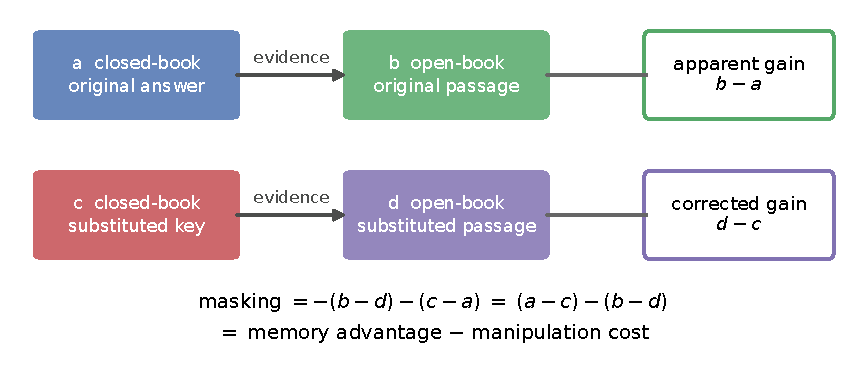
\includegraphics[width=\linewidth]{figures/fig1_method.pdf}
\caption{The four arms and what an apparent gain hides.
$\mask=(a-c)-(b-d)$: memory advantage minus manipulation cost.}
\label{fig:method}
\end{figure}

All accuracies use the project's frozen v3 scorer (answer-prefix stripping, first-sentence
extraction, DPR normalisation, strict EM), applied uniformly to every arm and every
subsequent re-analysis. Differences are tested with paired bootstrap over questions
($B{=}10{,}000$, seed \texttt{20260903}); question sampling from each pool uses the same
fixed seed, so every pair of conditions compared below sees an identical item set.

\subsection{Corpora and models}
\label{sec:corpora}
Both pools are built on public benchmarks: TriviaQA \citep{joshi2017} for single-hop
factoid questions and HotpotQA \citep{yang2018} for multi-hop questions.
Table~\ref{tab:corpora} summarises the resulting pools and their model coverage.
Throughout we name the construction version explicitly: \textbf{v0} is the original
construction, \textbf{v1} applies only the date-era fix, and \textbf{v2} applies both
fixes (numeric-boundary and date-era) and is the corpus behind \emph{every} headline
number; v0 and v1 appear only in ablations, labelled as such.
\begin{table}[t]\centering\small
\caption{Corpora (all on the final fixed construction, ``v2''). TriviaQA is single-hop
factoid; HotpotQA is multi-hop and has \emph{no} single-hop sub-population (every question
has two supporting paragraphs).}
\label{tab:corpora}
\begin{tabular}{llrr}
\toprule
Pool & Source / filter & $n$ & Models \\
\midrule
TriviaQA (C-line) & date/numeric answers, unique terminal hit & 432 & 5 Qwen3 \\
TriviaQA (B-line) & same pool, shared-corpus BM25 retrieval & 432 & 6 (incl.\ Qwen3.5) \\
HotpotQA (C-line) & year/numeric answers, unique terminal hit & 393 & 5 \\
\bottomrule
\end{tabular}
\end{table}
We use locally hosted Qwen3 models \citep{qwen3} (0.6B/1.7B/4B/4B-Instruct/8B) and, for a
cross-generation check, Qwen3.5-4B-Base.
% TODO(submission): Qwen3.5-4B-Base is a vision-language architecture and is therefore not
% modality-matched to the Qwen3 text models; the point is disclosed in Limitations. Add the
% Qwen3.5 technical-report citation once a citable reference exists.

% ============================================================================
\section{Validating the manipulation}
\label{sec:validity}
% ============================================================================

An effect measured on a flawed corpus is not an effect. We therefore audited the
manipulation before interpreting any result.

\subsection{Human audit}
We drew a deterministic, outcome-blind systematic sample of 90 items (20.2\% of the
446-item construction list handed to the annotators) and had two annotators independently judge, for each item,
whether the replacement was usable; disagreements were then re-checked by us against
character-level diffs of the original and modified passages.
Agreement is $\kappa{=}0.82$ over all 90 items and $0.78$ over the 86 both annotators
completed (the four initially-undecided items were resolved only after the annotators
conferred, which compromises their independence; we therefore report both readings and
treat the lower one as the conservative one).
\textbf{24.4\% (22/90) of items were invalid} (Table~\ref{tab:audit}, Fig.~\ref{fig:validity}a).

\begin{table}[t]\centering\small
\caption{Defect taxonomy from the human audit ($n{=}90$). \emph{Wrong position} means the
borrowed value was inserted at a coincidental occurrence---a date fragment, a citation
number, or another entity's value---rather than at the answer.}
\label{tab:audit}
\begin{tabular}{lrl}
\toprule
Class & \# & Example (index, old $\to$ new) \\
\midrule
wrong position & 17 & \texttt{August 4} $\to$ \texttt{August 7} (a birth date) \\
malformed value & 3 & year $1818$--$1848 \to$ \emph{``one thousand, two hundred and fifteen''} \\
new = true answer & 1 & $100{,}000 \to 100000$ (comma removed) \\
self-contradictory & 1 & \texttt{Apollo 11} $\to$ \texttt{Apollo 81} (while citing \texttt{AS-506}) \\
\midrule
total & 22 & \\
\bottomrule
\end{tabular}
\end{table}

\subsection{Root causes}
The 22 defects have three distinct causes. Seventeen take the form ``the plant landed on the
wrong occurrence''; the remaining five are defects of the planted value itself. We give the
counts so that the taxonomy in Table~\ref{tab:audit} and the causes here reconcile.

\paragraph{(i) A numeric boundary bug (4 of 22).} The uniqueness gate counts whole-token
occurrences using the character class $[0\text{--}9A\text{--}z]$, which excludes the decimal
point and the thousands separator. A value such as \texttt{3} therefore matches
\emph{inside} \texttt{2.3} or \texttt{7,100}, and the substitution lands in the middle of a
number. Fixing this (rejecting occurrences glued to a longer numeric expression) has 100\%
precision on the audited items (4/4 caught, 0/68 false positives) and removes 15 items
corpus-wide.

\paragraph{(ii) The ``a unique match locates the answer'' assumption (13 of 22).} The
construction assumes that if the answer string occurs exactly once in the passage, that
occurrence \emph{is} the answer, and plants there without asking the model to disambiguate.
The remaining thirteen wrong-position defects are this assumption failing: the unique
occurrence was a citation number, a date fragment, a count of something else, an entry in a
chronology, or a figure caption. We did \emph{not} fix this by rule---we could not find
one---and instead added an LLM span-verification probe, reported below as a weak filter
rather than a solution. It is the largest single source of invalid items.

\paragraph{(iii) The planted value is not credible, or not actually different (5 of 22).}
Three items render a borrowed year as English words (\emph{``one thousand, two hundred and
fifteen''}), one replaces $100{,}000$ by $100000$---the same number with the separator
removed---and one asserts \texttt{Apollo 81} while the same passage still cites
\texttt{AS-506}. The era constraint introduced for the gate in \S\ref{sec:gate3} attacks part
of this class by keeping borrowed years within 20 years of the original: the model in the
example above notices the contradiction (\emph{``the context says Scott Travis was born in
1876, but that's impossible because he was born in 1976''}) and then answers something that
is neither the planted value nor the remembered one. The constraint lowers the median
plant-to-original year gap from \textbf{69 to 7 years} with no item losing its candidate.

The two fixes are applied together. Their effect on pool size is exact and worth stating
plainly: the run pool before the fixes contains 447 items, the boundary fix removes 15 of
them, and the corpus used throughout this paper contains \textbf{432}. (The audit above was
drawn from a 446-item construction list, one item shorter than the run pool, so the audit
denominator and the run denominator are not the same number; we report both rather than
reconciling them post hoc.)

\subsection{Screening does not replace auditing}
We tested whether the audit can be automated. Three deterministic rules (lexical overlap
between question and the sentence containing the plant; adjacency to digits; proximity to
month names) catch 18/22 defects but mis-flag 47 of 68 good items (\textbf{69\% false
positive}): unusable. An LLM verifier asked to judge the marked occurrence reaches only
\textbf{45\% recall at 4.4\% false positive}. Applied corpus-wide it flags 43/446 items,
at a rate that matches between the audited sample (11.1\%) and the rest (9.3\%), implying a
corpus-level defect rate of $\approx 22.7\%$---consistent with the human estimate of
24.4\%. \textbf{Human auditing is not optional.}

\subsection{Cleaning does not change the conclusions}
We recompute the whole analysis on the fixed corpus with every audited defect removed---the
22 items the human audit judged invalid and the 43 the model probe flagged (56 distinct
items, all in the TriviaQA pools). \textbf{All 20 model$\times$line$\times$depth cells keep
their sign and their significance}, and the TriviaQA scale curve is unchanged in shape
(Table~\ref{tab:app-cleaning}); the effect is if anything slightly larger after cleaning, as
it was on the pre-fix corpus, i.e.\ the bad items dilute the effect rather than create it.
On the reference B-line model the pre-fix corpus moves from $0.184$ to $0.257$ at $k{=}1$
and from $0.090$ to $0.176$ at $k{=}5$ (Fig.~\ref{fig:validity}c).

\paragraph{The direction of these defects matters, and it is in our favour.}
The usual hazard of a constructed corpus is that defects \emph{manufacture} an effect. Here
they act the other way, and the reason is visible in the identity. A model that rejects an
implausible plant answers neither the planted value nor the original one, so it scores wrong
on the substituted key; that inflates the manipulation cost $(b-d)$ and therefore
\emph{shrinks} $\mask=(a-c)-(b-d)$. Our measured effect is thus biased \emph{against} the
claim, not for it---and that is what we observe: every fix we have made has moved masking up
rather than down (C-line 8B: $0.166 \to 0.232$; B-line 8B: $0.184 \to 0.257$; the HotpotQA
oracle drop: $13.2\% \to 1.5\%$). This is why we treat the audit as strengthening the result
rather than undermining it, and why remeasuring after cleaning leaves the cells where they
were rather than cancelling them. It does \emph{not} license the assumption that every
unfixed defect behaves this way: the residual class described in \S\ref{sec:validity} is
untested, and we report it as an open quantity rather than as a known-conservative one.
The HotpotQA pools are unaffected by construction, because the audit was drawn from the
TriviaQA pool; we therefore report the cleaning result as a TriviaQA robustness check, not
as evidence about multi-hop behaviour.

\begin{figure}[t]\centering
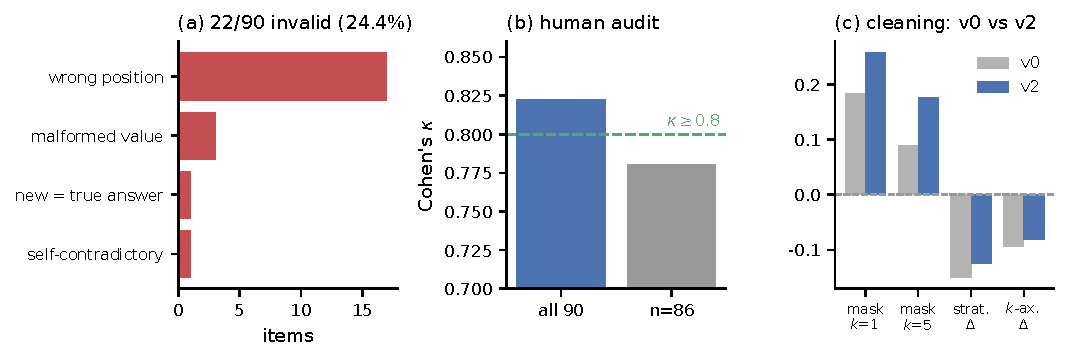
\includegraphics[width=\linewidth]{figures/fig2_validity.pdf}
\caption{Validating the manipulation. (a) Defect classes in the 90-item audit;
(b) annotator agreement (both readings, threshold marked); (c) cleaning the corpus does not
change the conclusions---it strengthens masking.}
\label{fig:validity}
\end{figure}

\subsection{Entity answers: an active constraint that changes nothing}
\label{sec:entity}

Our pools are restricted to numeric and date answers because those are the shapes a
type-consistent borrowing rule can control. Entity-type answers are at least as common a
target of substitution probes \citep{longpre2021entity}, so we ask whether the boundary
located in \S\ref{sec:precond} is about question difficulty or about the \emph{form} of the
answer. We built a pool of $1{,}067$ entity-answer questions (a name-type answer that occurs
exactly once as a whole token in the final gold passage), drew a deterministic $400$-item
sample, and ran the four-arm design on the identical items and models under two borrowing
rules: the unconstrained rule, which buckets every entity answer together, and a
\emph{domain-consistency} rule. The rule needs no named-entity recogniser: each question gets
a signature of six words that are neither unique to it nor ubiquitous (document frequency in
$[2,8\%]$ of the pool, taken in decreasing frequency), and a candidate is accepted if its
source question shares at least two signature words and its answer falls in the same
token-count band. The requirement is relaxed level by level (one shared word, then band only,
then the unconstrained bucket), so no item can lose its candidate.
$363$ items were constructed in every condition; the $37$ losses are items where the answer
is not a whole-token match in some gold passage and are identical across all four runs.

\paragraph{Auditing the new construct was necessary, and instructive.}
The first pass of this experiment looked like a success: compliance rose from $0.091$ to
$0.174$ (4B-Instruct) and from $0.127$ to $0.220$ (8B), oracle drop fell, and masking rose
significantly. All of it was an artifact of the new rule, in three ways that we found only by
auditing the construct we had just built---each of them biasing \emph{towards} the rule
looking good.
\emph{(i) The rule was not deterministic.} Signature words were ranked by document frequency
alone; ties (which are numerous) were then broken by Python set-iteration order, which is
randomised per process. Two runs over the same items therefore planted different values for
$117$ of $363$ items, and the two models' substitution files differed although the rule does
not depend on the model at all.
\emph{(ii) $13.5\%$ of plants were the same value in another spelling} (\emph{Wagner}
$\rightarrow$ \emph{Wagners}, \emph{St.~Louis} $\rightarrow$ \emph{st louis}).
\emph{(iii) $62.0\%$ and $61.2\%$ of items received a plant that is simply another entry in
the \textbf{target question's own answer list}}. TriviaQA lists a median of $11$ accepted
answer strings per question (mean $15.6$, maximum $183$), and the same-pool borrow sees all
of them; the most topically similar candidate to a question is its own answer under another
name, so the constraint selected precisely those. The unconstrained rule, drawing
near-randomly from about a thousand candidates, produced \emph{zero} such items. This is the
mechanism behind the first-pass result: a plant that is another name for the true answer
raises the closed-book arm on the substituted key and the open-book substituted arm at the
same time, which is exactly what a positive masking result looks like.

We guarded against all three---a total order on the signature ranking, and rejection of
candidates that are a surface variant of the original or appear in the target question's own
answer list, in both cases as a preference so that no item loses its candidate---and re-ran.
With the guards, closed-book accuracy on the planted key is exactly $0.000$ in both models,
and the first-pass effects disappear (Table~\ref{tab:entity}).

\begin{table}[t]\centering\small
\caption{Entity-answer pool ($n{=}363$). Masking is \emph{negative} in all four cells
(significantly so in three; the constrained 4B-Instruct interval touches zero). A negative
value means the manipulation cost exceeds the memory advantage: the substitution does not
suppress the open-book gain at all. We attribute that to the scoring asymmetry and to the
difficulty of reading a substituted entity rather than to a measured positive effect, and
\S\ref{sec:entity} states what that leaves open. The single-variable contrast between the
two rules is indistinguishable from zero. The domain-consistency rule is verifiably active:
$24.5\%$ of items were satisfied at its strictest level, $70.0\%$ at the second, $5.5\%$ at
band-only, and none fell back to the unconstrained bucket.}
\label{tab:entity}
\begin{tabular}{llcccccc}
\toprule
Rule & Model & $a$ & $b$ & $c$ & $d$ & \mask\ (95\% CI) & $\Delta\mask$ \\
\midrule
unconstrained      & Qwen3-4B-Instruct & 0.198 & 0.350 & 0.000 & 0.091 & $-0.061$ [$-0.116$, $-0.003$] & --- \\
domain-consistent  & Qwen3-4B-Instruct & 0.198 & 0.350 & 0.000 & 0.094 & $-0.058$ [$-0.116$, $+0.000$] & $+0.003$ [$-0.030$, $+0.036$] \\
unconstrained      & Qwen3-8B          & 0.298 & 0.537 & 0.000 & 0.124 & $-0.116$ [$-0.176$, $-0.052$] & --- \\
domain-consistent  & Qwen3-8B          & 0.298 & 0.537 & 0.000 & 0.154 & $-0.085$ [$-0.149$, $-0.022$] & $+0.031$ [$-0.008$, $+0.069$] \\
\bottomrule
\end{tabular}
\end{table}

\paragraph{What this buys, and what it does not.}
The constraint is active on essentially every item, and it changes nothing: masking stays
\emph{negative} under both rules---significantly so in three of the four cells (both
unconstrained cells and the constrained 8B cell), while the constrained 4B-Instruct interval
touches zero---so the rule does not restore the effect we set out to restore, and the paired
contrast between the two rules is $+0.003$ and $+0.031$ with intervals that include zero
(compliance and oracle drop move by the same insignificant amounts in the same directions).
Read together with \S\ref{sec:precond}, the boundary is therefore about the
\emph{shape of the answer} rather than about multi-hop difficulty: the effect appears where
the answer is a value a model can have memorised as a chunk, and we have not been able to
produce it on entity answers by making the manipulation more credible. Whether a different
construction could is open; what we can say is that this one, audited properly, cannot.
The guard decision matters for reproducibility and we state it: the guards apply only inside
the constrained branch, so every number reported elsewhere in this paper reproduces
bit-for-bit, the unconstrained entity arm reproduces its artifacts item by item ($363/363$),
and the two constrained runs now produce byte-identical substitution files.

\paragraph{Robustness of the entity result to the two known biases.} Both biases we
identified can be attacked with the data in hand, and we did, so that the entity conclusion
does not rest on them. The first is the scoring asymmetry: the substituted-arm cells are
scored against a single canonical key while the original-answer cells use the full answer
list. We rescored the substituted arms against the planted value's own answer forms, taking
care to drop any form that also appears in the \emph{target} question's answer list (which
would credit the true answer, i.e.\ over-correct). The second is pool contamination: $32$ of
the $363$ sampled items ($82$ of the $1{,}067$ in the full pool) have an answer that contains
digits or a question that also appears in the numeric/date pool, so we recomputed the arm on
the remaining $331$. Table~\ref{tab:entity-robust}
reports both. The conclusion is stable: masking remains negative under every variant, i.e.\ we
never observe positive masking on entity answers, and no variant brings the rule contrast to
a point where we would read it as restoring the effect. What the variants move is the
\emph{depth} of the negative value---and, for 8B, whether the rule contrast is distinguishable
from zero at all ($+0.031$ with the uniform scorer, $+0.044$ under alias-aware rescoring,
$+0.033$ on the cleaned pool). We report the uniform scorer as primary because every other
number in the paper uses it, and we report the alternatives rather than choosing the one that
suits the narrative. One thing we cannot claim, and one thing we now can. We have not
localised the residual negative value to zero: after removing the two biases above it sits at
$-0.03$ to $-0.07$ rather than at zero. But a deterministic 52-item sample of the arm (every
seventh item) rules out the explanation we thought most likely. None of the 52 planted values
was the same entity under a name absent from the target's answer list, so that class is small
at most ($0/52$; upper bound $\approx 6\%$ by the rule of three). What the same sample does
show is a different failure mode: the topical signature matches \emph{subject matter}, not
\emph{answer kind}, so the plant is often not of the kind the question asks for---a city where
a count is wanted, an abstract phrase where a character name is wanted, a person where the
number of planets is wanted. Judged by a single annotator (one of us) on those 52 items, about
two thirds of the plants are of a different kind from the gold answer, and those are the items
where a model is most likely to answer neither the planted value nor the original. That is the
mechanism we would attack next, with an explicit answer-type constraint rather than a topical
one. The sign we report does not depend on it, and the single-annotator judgement is the
weakest evidence in this subsection.

We implemented that fix and validated it offline, and it is only a partial one. The constraint
accepts a candidate only if the question that supplies it asks for the same kind of answer, by
a wh-bucket rule (\emph{how many}/\emph{how much}, \emph{which year}, \emph{who},
\emph{which city/country}, \emph{which album/film/book}, \dots). On a $200$-item offline replay
it costs nothing---all $200$ items still borrow, none self-borrows, none is a same-value
plant---and raises strict bucket agreement from $49\%$ to $57\%$ and agreement on the
numeric axis from $96.5\%$ to $99.0\%$. The reason it is only partial is visible in the same
replay: $65.5\%$ of the questions in this pool fall outside the bucket system altogether
(\emph{Which is\ldots}, \emph{What was\ldots}), so for two thirds of the items there is no
type to match. We therefore do not report the constrained arm as a result; we report the
measurement that shows why a topical rule cannot be repaired by a wh-bucket rule, and we leave
a proper type system---or a named-entity model---to future work.

\begin{table}[t]\centering\small
\caption{The entity arm under three scoring/selection variants ($n$ as shown; the same items
in both arms of a row). Masking is negative in every variant, so no variant yields positive
masking; the variants move its depth, and for 8B whether the rule contrast is distinguishable
from zero.}
\label{tab:entity-robust}
\begin{tabular}{lllrr}
\toprule
Variant & Model & $n$ & \mask\ (95\% CI) & $\Delta\mask$, new $-$ old \\
\midrule
uniform scorer (primary) & 4B-Instruct & 363 & $-0.058$ [$-0.116$, $+0.000$] & $+0.003$ [$-0.030$, $+0.036$] \\
uniform scorer (primary) & 8B & 363 & $-0.085$ [$-0.149$, $-0.022$] & $+0.031$ [$-0.008$, $+0.069$] \\
alias-aware rescoring & 4B-Instruct & 363 & $-0.058$ [$-0.119$, $+0.000$] & $-0.006$ [$-0.039$, $+0.028$] \\
alias-aware rescoring & 8B & 363 & $-0.066$ [$-0.130$, $+0.000$] & $+0.044$ [$+0.006$, $+0.085$] \\
pool cleaned of numeric-form and overlapping items & 4B-Instruct & 331 & $-0.033$ [$-0.094$, $+0.027$] & $+0.003$ [$-0.030$, $+0.036$] \\
pool cleaned of numeric-form and overlapping items & 8B & 331 & $-0.048$ [$-0.115$, $+0.018$] & $+0.033$ [$-0.006$, $+0.076$] \\
\bottomrule
\end{tabular}
\end{table}

Two disclosures follow from this audit. First, the same trap exists in the other corpora,
and its rate tracks the size of the answer list, which is the quantity that makes it possible
(Table~\ref{tab:trap}). We can state it as a check that anyone building a substitution corpus
from a shared pool can run in one line: \emph{reject a candidate whose normalised form appears
in the target question's own answer list}. HotpotQA, whose pool stores a single answer string
per question, produces no such items; TriviaQA's numeric/date pool (median two accepted forms)
produces two per run ($0.46\%$ of items), and removing them moves every masking value by at
most $0.003$; the entity pool, with a median of eleven accepted forms, produced $61.6\%$ under the
topical constraint before we guarded against it and none after. Second, the substituted-arm
cells score against a single
canonical key while the original-answer cells score against the full answer list; the
asymmetry inflates the manipulation cost and therefore biases the entity-line masking
\emph{downward}, in the direction of the null we report. We keep the uniform scorer as
primary rather than compensating in every table, which would over-credit (it would count the
true answer as a hit whenever the plant is a synonym); the alias-aware rescoring above is the
robustness check for exactly this concern.

\begin{table}[t]\centering\small
\caption{The ``no-op substitution'' trap by corpus, measured over every frozen substitution
file with one check: a planted value is a no-op if its normalised form is another accepted
spelling of the \emph{target} question's own answer. The rate tracks the size of the answer
list, which is what makes the trap possible: pools with one accepted form per question cannot
produce it, and the constraint-driven entity rule produced it for most items until guarded.}
\label{tab:trap}
\begin{tabular}{lrrr}
\toprule
Corpus & answers/question (median) & substitutions examined & no-op plants \\
\midrule
HotpotQA, numeric/date & 1 & 1965 & $0.00\%$ \\
TriviaQA, numeric/date & 2 & 7344 & $0.46\%$ ($2$ per run) \\
TriviaQA, entity (unconstrained rule) & 11 & 726 & $0.00\%$ \\
TriviaQA, entity (domain constraint, before guard) & 11 & 726 & $61.6\%$ \\
TriviaQA, entity (domain constraint, after guard) & 11 & 726 & $0.00\%$ \\
\bottomrule
\end{tabular}
\end{table}

\subsection{The oracle-answerability gate is mis-specified}\label{sec:gate3}
A standard validity gate asks whether accuracy drops when the gold evidence is rewritten:
if the model cannot answer the new value even with the passage in hand, the item is judged
unusable. The gate's frozen thresholds are a drop of at most 3\% for GO, up to 8\% for
REVISE, and more than 8\% for ABANDON. On the fixed corpus it passes HotpotQA---reference
model drop $1.5\%$ ($13.2\%$ before the era fix), cross-generation model $2.5\%$---but on
TriviaQA it still returns ABANDON ($22.9\%$).
Decomposing the residual explains why: on the preceding (v1) corpus, of the 104 TriviaQA
items this gate flagged, 79 answer the remembered value rather than the planted one. We read
that residual as the treatment effect rather than as a corpus defect. We therefore argue
the gate should not be used in studies of memory--context
conflict: it aggregates \emph{evidence unusable} with \emph{model resistant}, which this
design needs to keep separate.

% ============================================================================
\section{Results}
% ============================================================================

\subsection{Masking is large and grows with scale}
Figure~\ref{fig:scale}a and Table~\ref{tab:cline} show masking on the TriviaQA C-line pool.
It is positive for all five models, significant for four, and its point estimate rises at
every step of the scale axis ($k{=}1$: $0.032 \to 0.095 \to 0.134 \to 0.213 \to 0.231$),
with no reversal; two of the four adjacent steps are individually significant
($0.6$B$\to1.7$B and $4$B$\to4$B-Instruct), and the other two have intervals that contain
zero. The smallest model (0.6B) is the only non-significant
point, and it has no memory to leak (closed-book $a{=}0.10$). Because these are five tests of
the same hypothesis on the same pool, we also apply a Holm correction across the five models
(exact paired sign tests on the item-level DiD, family $\alpha{=}0.05$): the four models at
$1.7$B and above survive ($p_{\mathrm{Holm}} \le 0.0007$) and 0.6B does not ($p{=}0.154$),
so the correction changes no statement in this subsection.

\begin{figure}[t]\centering
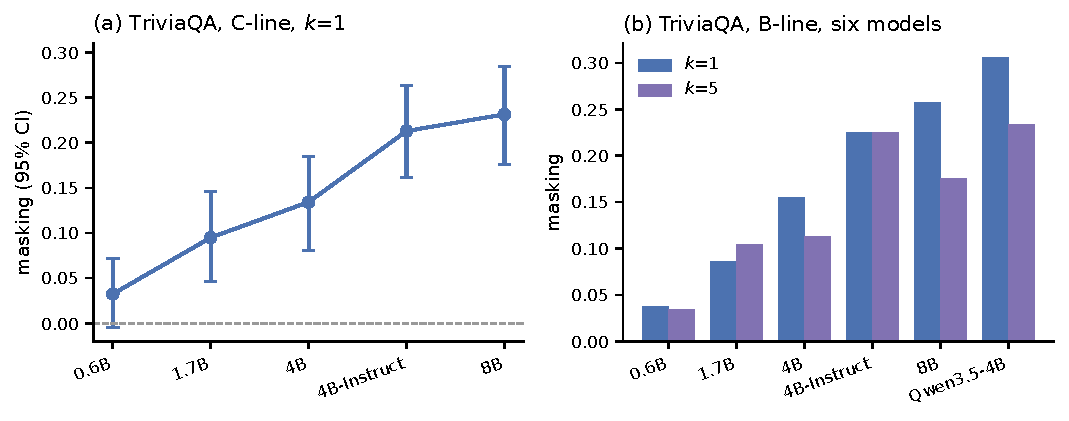
\includegraphics[width=\linewidth]{figures/fig3_scale.pdf}
\caption{Masking and model scale. (a) TriviaQA C-line, $k{=}1$, 95\% CI: the point estimate
rises at every step, and the claim is limited to $k{=}1$. (b) B-line, six models, both $k$;
$k{=}1$ is monotone in scale, $k{=}5$ has one reversal (8B below 4B-Instruct).}
\label{fig:scale}
\end{figure}

\begin{table}[t]\centering\small
\caption{TriviaQA C-line, final construction (v2), $n{=}432$ questions, v3 scorer,
paragraph granularity, context budget 1024 tokens, greedy decoding at 4-bit quantisation;
all four arms are measured on the same items. Readers can verify $\mask=(a-c)-(b-d)$ from
the row itself. Masking CIs are the reflection of the paired DiD CI.}
\label{tab:cline}
\begin{tabular}{lrrrrr}
\toprule
Model & $a$ & $b$ & $c$ & $d$ & \mask\ (95\% CI) \\
\midrule
Qwen3-0.6B        & 0.102 & 0.502 & 0.009 & 0.442 & $+0.032$ \,[$-0.005$, $+0.072$] \\
Qwen3-1.7B        & 0.213 & 0.424 & 0.009 & 0.315 & $+0.095$ \,[$+0.046$, $+0.146$] \\
Qwen3-4B          & 0.382 & 0.690 & 0.012 & 0.454 & $+0.134$ \,[$+0.081$, $+0.185$] \\
Qwen3-4B-Instruct & 0.363 & 0.562 & 0.007 & 0.419 & $+0.213$ \,[$+0.162$, $+0.264$] \\
Qwen3-8B          & 0.472 & 0.664 & 0.007 & 0.431 & $+0.231$ \,[$+0.176$, $+0.285$] \\
\bottomrule
\end{tabular}
\end{table}

\paragraph{An old anomaly was an artifact.} On the pre-fix corpus the scale ordering was
non-monotone: 1.7B showed \emph{more} masking than 4B. On the fixed corpus that reversal
disappears, and the change in that step is itself significant (interaction
$\Delta{=}{+}0.065$, 95\% CI $[{+}0.019,{+}0.111]$). We report this carefully: the reversal
was never individually significant on either corpus; what is significant is that fixing
the manipulation moved the step.

\subsection{The decomposition, and a prediction that failed}
\label{sec:precond}
Equation~\eqref{eq:decomp} is an exact identity, so it cannot be tested as a hypothesis. It
is nevertheless informative, because one of its two terms is pinned near the floor by
construction: the closed-book arm on the substituted key has the same input as the
closed-book arm on the original---the substitution is invisible to a model that sees no
passage---and the borrowed value comes from a different question, so the model almost never
produces it spontaneously ($c \in [0.005, 0.021]$ across every pool and model we ran). The memory advantage
$(a-c)$ is therefore close to $a$ itself, and the only term that can move under a change of
setting is the manipulation cost $(b-d)$. Table~\ref{tab:decomp} lists both terms on
Qwen3-8B for the two pools, and Figure~\ref{fig:precond}a plots them:

\paragraph{The identity, seen item by item.} Because the identity fixes the behaviour of
$(a-c)$ once $a$ is known, it makes a sharp prediction at the item level, and we check it
rather than assert it: split each run's items by whether the model answered correctly
closed-book ($a{=}1$) or not ($a{=}0$). Masking is strongly positive on the $a{=}1$ items
($+0.50$ to $+0.95$ across our 20 model$\times$line cells) and slightly \emph{negative} on
the $a{=}0$ items ($-0.02$ to $-0.17$). This is the identity at work, not an independent
discovery---the gap between the two strata is bounded near $1$ by construction, since $a$
differs by exactly $1$ between them---and we report it as such
(Table~\ref{tab:app-conditional}). Its value is diagnostic: it confirms that the quantity we
call masking lives entirely on the questions the model could already answer, which is the
boundary \S\ref{sec:precond} is about.

\begin{center}\small
\captionof{table}{The two terms of Equation~\eqref{eq:decomp} on Qwen3-8B, both pools, on
the final construction. Both are accuracy differences, not accuracies.}
\label{tab:decomp}
\begin{tabular}{lccc}
\toprule
Pool & memory advantage $(a-c)$ & manipulation cost $(b-d)$ & \mask \\
\midrule
TriviaQA ($n{=}432$) & $+0.465$ & $+0.234$ & $\mathbf{+0.231}$ \\
HotpotQA ($n{=}393$) & $+0.046$ & $+0.053$ & $\mathbf{-0.008}$ \\
\bottomrule
\end{tabular}
\end{center}

On multi-hop questions the model simply does not have the answer in memory
(closed-book $a$ is $0.01$--$0.06$ across the five), so there is little advantage to leak. We do
not claim the effect
is exactly zero here---only that it is not detected. To say something stronger we run an
\emph{equivalence test} (TOST, $\alpha{=}0.05$) on the paired DiD: for all five HotpotQA
models the 90\% interval lies inside $\pm 5$ accuracy points, so we can reject effects of
that size, while the 95\% interval half-width is $2.5$--$3.6$ points, so we cannot exclude
effects up to roughly $3.5$ points (Fig.~\ref{fig:precond}b). The margin $\delta{=}5$ points
is chosen before the test as the smallest effect we would be willing to call practically
meaningful for a per-configuration accuracy difference; we report the
half-width alongside it so that a reader who prefers a tighter margin can see exactly what
is and is not excluded.

\paragraph{The precondition, measured rather than asserted.} The identity also tells us how
to test the precondition quantitatively. Write masking as a function of the model's
closed-book accuracy $a$. If the closed-book arm on the substituted key sat at the floor
\emph{and} the manipulation cost were constant, the identity would force
$\mask\approx a-\text{const}$, i.e.\ a slope of exactly $1$. Across the $17$
model$\times$line$\times$depth cells that share the numeric/date corpus the fitted slope is
$0.50$ (intercept $-0.013$; $0.52$ on the C-line, $0.50$ on the B-line), with a 95\% interval
of $[0.44,0.57]$ from resampling items within each cell and a range of $0.48$--$0.52$ under
leave-one-model-out; the slope is below $1$ in every one of the $10{,}000$ bootstrap
replicates. The shortfall is the informative part: as models become better at the task the
manipulation cost $(b-d)$ rises as well, so only about half of the memory advantage reaches
masking. The same relation shows up \emph{within} the pool: the date sub-pool has the higher
closed-book accuracy in the four larger models and also the larger masking ($0.184$ vs
$0.076$ at 4B, $0.299$ vs $0.111$ at 4B-Instruct, $0.368$ vs $0.071$ at 8B; the two smallest
models are indistinguishable), so the ordering is not an artifact of pooling dates with
numbers. HotpotQA sits at the low-$a$ end of the same ordering ($a\le0.06$, masking
$\approx0$). The entity pool now has three points, and they fall away from the curve as $a$
grows: at $a{=}0.11$ (Qwen3-1.7B) its masking is $+0.02$ with an interval containing zero, close
to the curve's $+0.04$; but at $a{=}0.20$ and $a{=}0.30$ it is $-0.06$ and $-0.09$ where the curve
predicts $+0.09$ and $+0.14$. That is why we report it separately and with the caveats of
\S\ref{sec:entity} rather than as a point on the
curve. One attempt to break the mechanical link directly gives a partial answer. We
replaced the binary indicator with continuous within-model measures that enter none of
$a,b,c,d$. The closed-book log-probability of the true answer predicts masking on its own
($+0.069$, 95\% CI $[0.056,0.086]$) but adds nothing once the binary closed-book indicator is
controlled for ($-0.003$, $[-0.012,0.005]$), and it does not explain the manipulation cost
either ($+0.001$, $[-0.007,0.009]$). The \emph{margin} between the true and the planted
answer's log-probability does add a little in both places ($-0.013$, $[-0.021,-0.005]$ on
masking; $+0.016$, $[+0.008,+0.024]$ on the manipulation cost), i.e.\ in the direction the
identity requires---but that coefficient is two orders of magnitude smaller than the binary
indicator's, and we tried this operationalisation \emph{after} the level measure came out null,
so we report it as exploratory. We therefore read the dose--response as an identity-adjacent
diagnostic of \emph{where} masking can live, with at most a small independent component.

\paragraph{Why the manipulation cost rises with memory.} The mechanism behind the slope is
visible item by item. Define an item's memory strength \emph{without} the model being scored:
for model $m$ and item $i$, take the number of \emph{other} models in the same pool that
answer $i$ correctly closed-book, so the strength variable cannot be a restatement of $m$'s own
closed-book accuracy. The manipulation cost $(b-d)$ then increases with that
strength in all six models, and by a large factor: $+0.03 \to +0.82$ for 8B,
$+0.12 \to +0.76$ for Qwen3.5-4B, $+0.07 \to +0.71$ for 4B, $+0.04 \to +0.50$ for
4B-Instruct, $+0.02 \to +0.52$ for 1.7B and $+0.03 \to +0.31$ for 0.6B
(Table~\ref{tab:strength}). The rise is not bin-by-bin monotone---only 4B is strictly
monotone across the six bins, and 0.6B dips to $-0.04$ at strength $1$---so we report it with
two summaries that do not depend on how the bins are cut: the extreme contrast between
strength $5$ and strength $0$ is $+0.27$ to $+0.80$ with a 95\% item-bootstrap interval
excluding zero in all six models, and the item-level rank correlation between strength and
$(b-d)$ is positive with an interval excluding zero in all six (the same two summaries are
weaker but still positive at $k{=}5$). Items that many models know are exactly the items where replacing
the answer costs the most, because the model has something to fall back on; items nobody knows
are read off the passage almost regardless of what it says. That is why the memory advantage
does not translate one-for-one into masking, and it is a property of the items, not of any one
model.

\begin{table}[t]\centering\small
\caption{Manipulation cost $(b-d)$ by memory strength, where an item's strength is the number
of \emph{other} models in the pool that answer it correctly closed-book (strength $5$ means
all five others do). Strength is defined without the scored model, so the relation is not a
restatement of its own closed-book accuracy. Cell sizes are $17$--$146$ items; only the
extremes are shown, and the intermediate bins are \emph{not} monotone for five of the six
models (see the text for the summaries we rely on instead).}
\label{tab:strength}
\begin{tabular}{lrrrr}
\toprule
 & \multicolumn{2}{c}{$(b-d)$} & & \\
\cmidrule(lr){2-3}
Model & strength 0 & strength 5 & ratio & $n$ (0 / 5) \\
\midrule
Qwen3-0.6B     & $+0.033$ & $+0.308$ & $9\times$  & 120 / 39 \\
Qwen3-1.7B     & $+0.024$ & $+0.524$ & $22\times$ & 124 / 21 \\
Qwen3-4B       & $+0.065$ & $+0.714$ & $11\times$ & 123 / 21 \\
Qwen3-4B-Instruct & $+0.040$ & $+0.500$ & $13\times$ & 126 / 18 \\
Qwen3-8B       & $+0.028$ & $+0.824$ & $29\times$ & 143 / 17 \\
Qwen3.5-4B-Base & $+0.116$ & $+0.765$ & $7\times$  & 146 / 17 \\
\bottomrule
\end{tabular}
\end{table}

\begin{figure}[t]\centering
\caption{The decomposition. (a) Memory advantage vs manipulation cost for Qwen3-8B on two
pools; masking is their difference. (b) On HotpotQA all models' DiD is indistinguishable
from zero, and an equivalence test excludes effects above five points. (c) The
cross-generation memory gain is confined to single-hop questions (y-axis: closed-book
accuracy $a$, not masking).}
\label{fig:precond}
\end{figure}

\paragraph{Pre-registered cross-generation test.} The identity licenses exactly one
falsifiable extrapolation: if we scale the model up, $(a-c)$ should rise, and on a pool
where the two terms currently balance (HotpotQA) that should tip masking into existence. We
pre-registered this and \textbf{it failed}. Qwen3.5-4B-Base gains a large memory advantage
over Qwen3-4B on TriviaQA ($a$: $0.382 \to 0.558$, $+0.176$; on the same 432 questions,
165 and 241 correct, overlapping on 143, for a net $+76$), but on HotpotQA the two are
indistinguishable ($0.056 \to 0.056$: 22 correct either way, overlapping on only 9, net
$0$). The boundary is therefore sharper than our hypothesis: \textbf{it
is not how much memory a model has, but whether the particular question is in
memory}---and a stronger model does not remove it. Two caveats bound how far this can be
pushed. It is a single model pair, and the two models differ in more than generation:
Qwen3.5-4B-Base is a vision-language architecture and was run under a different library
version, so we cannot separate a generation effect from a modality or implementation
effect. And the sentence above is our reading of a failure, not a pre-registered outcome.
We therefore report this as a \emph{descriptive contrast} that sharpens the boundary, and
not as a confirmation of it.

\subsection{The decision axis (an instance)}
\label{sec:decision}
Top-$k$ depth is one decision this contamination can distort. On the B-line (shared-corpus
BM25 retrieval, $k \in \{1,5\}$, six models), masking is positive in \emph{all} 12 cells and
its 95\% interval excludes zero in \textbf{10} of them---the two exceptions being both cells
of the 0.6B model, whose closed-book floor leaves nothing to leak (Table~\ref{tab:app-bline}
reports every cell with its interval). Within the compliance
stratum the corrected gain is higher at $k{=}1$ than at $k{=}5$ for \textbf{6/6} models.
Throughout this paper $\Delta_{\text{strat}}$ is written as $k{=}5$ \emph{minus} $k{=}1$, so
a negative value means $k{=}1$ is better ($-0.09$ to $-0.41$; every 95\% interval excludes
zero). Because six models are six replications of one contrast rather than six independent
hypotheses, we also apply Holm correction to the exact paired sign tests across the six
primary tests: all six survive it (largest adjusted $p = 0.034$).

\paragraph{What we do not claim.} We looked for a decision that the correction robustly
\emph{reverses} at the full-sample level---the strongest form of the claim this paper could
make---and we did not find one, so we do not make it. The full-sample $k$ comparison is
significant in only 2/6 models; the stratum result above is robust under Holm, under
leave-one-model-out and under clustered resampling, but its \emph{significance} is
conditional on a post-hoc cut (under the construction-based cut it is significant in 1/6).
We also tried the model-selection decision---choosing the best model by apparent versus by
corrected gain changes which model wins, and shuffles the rest of the ranking---but the
argmax changes in only $0.679$ of paired bootstrap resamples ($0.688$ if configurations are
resampled independently), below the $0.80$ threshold
this project uses elsewhere. The honest summary is that the correction moves
\emph{magnitudes} in the same direction for all six models---a 9-to-41-point shift---and
\emph{rankings} only weakly, and we report it as such. We therefore treat this axis as
\emph{exploratory}: the contribution of the paper is the measurement protocol, the audit of
the manipulation, and the boundary---not a recommendation about which configuration to
deploy, which would need a decision that survives the full sample.

\paragraph{What does change: which configurations clear a practical bar.} A developer rarely
asks whether $k{=}1$ beats $k{=}5$ significantly; they ask whether a configuration is worth
deploying at all, i.e.\ whether its gain clears some practical threshold. That question
\emph{is} affected, and in one direction: because masking is positive in every B-line cell,
the corrected gain is always the larger of the two, so screening by apparent gain
systematically \emph{under-admits}. At a $5$-point bar nothing changes; at $10$ points two of
the twelve configurations ($1.7$B $k{=}5$ and 8B $k{=}1$) cross the bar once corrected; at
$20$ points six do; at $25$ points eight do. The per-model choice of depth changes as well:
on point estimates the apparent gain prefers $k{=}5$ in four of six models and $k{=}1$ in
two, while the corrected gain prefers $k{=}1$ in five of six, so the choice flips in three
models (4B, 8B, Qwen3.5-4B). We report this as a consequence of a positive masking level and
not as a significance claim: the individual full-sample differences remain significant in
only 2/6 models, and nothing here licenses a recommendation about which depth to deploy.

\paragraph{The decision that does reverse.} There is one decision rule we can say the
correction reverses, and we state it with its caveats rather than as a headline. Take the
practical question ``which configuration should we deploy?'' and answer it by the rule a
practitioner would actually use---pick the configuration with the largest measured gain. On
the B-line space of six models $\times$ two depths, the largest \emph{apparent} gain belongs
to the \emph{smallest} model at the larger depth ($0.6$B, $k{=}5$: $+0.333$), while the
largest \emph{corrected} gain belongs to the cross-generation model at the smaller depth
(Qwen3.5-4B-Base, $k{=}1$: $+0.442$); the argmax changes in $\mathbf{0.999}$ of $10{,}000$
paired bootstrap resamples ($0.997$ if configurations are resampled independently), and
$0.999$ for the model choice alone if each model is allowed its better
depth ($0.994$ independently). The mechanism is visible across the twelve configurations: the apparent gain
correlates \emph{negatively} with the model's closed-book accuracy ($r{=}-0.51$), because a
weak no-evidence baseline inflates it, while the corrected gain correlates positively
($r{=}+0.50$). The apparent gain therefore rewards the model that knows least, and the
correction removes that reward. Two caveats bound what this is worth. It is a
point-estimate decision rule, not a significance claim: the pre-registered criterion above,
which requires the corrected gains to separate, still fails. And we chose this rule after
seeing the data, so it is exploratory; what we can defend is that the reversal is stable,
mechanically explicable, and undiminished by the resampling.

The compliance stratum is a \emph{post-hoc} cut, chosen after we had inspected the full
data; the paired-difference criterion applied inside it was frozen before the re-run
reported here, but the stratum itself was not pre-registered. Readers should weight the
full-sample numbers reported below accordingly, and we report both throughout.

\paragraph{Two robustness checks on the stratum.} Because the cut is post-hoc, we vary it.
Under the \emph{broadest} definition---the planted value merely occurs in the retrieved
context---the paired difference is negative in all six models but significant in only one;
under the two stricter definitions used above, which additionally require that the model
actually adopted the planted value, it is significant in all six. Across the 18
model$\times$definition cells the sign never flips. We therefore report the
\emph{direction} as robust and treat the \emph{significance} of the $k$ comparison as
conditional on the stratum. Separately, dropping any single model from the pooled stratum
leaves the pooled difference between $-0.12$ and $-0.16$ with intervals excluding zero, and
resampling whole borrowed values rather than questions---the same planted value can recur
across items---moves every interval by at most $0.015$
(Tables~\ref{tab:sens} and~\ref{tab:cluster}).

We deliberately \emph{do not} headline the $k$ comparison itself---that is, the claim that
$k{=}1$ beats $k{=}5$ inside the stratum. We do report, and do headline, the weaker and
simpler fact that masking is positive in every retrieval cell. Its magnitude is unstable under
methodological cleanup ($-0.094$ pre-fix, $-0.059$ under one restriction, $-0.097$ under
another, $-0.081$ on the fixed corpus), and on the fixed corpus only 2/6 models show a
significant full-sample gap. We report it as one instantiation of a decision axis, and we
report the weaker secondary criteria alongside the primary one (marginal-CI separation:
2/6).

\begin{table}[t]\centering\small
\caption{B-line, final construction (v2), $n{=}432$, all six models. $\Delta_{\text{strat}}$
is the paired $k{=}5$ \emph{minus} $k{=}1$ difference in corrected gain inside the
compliance stratum, so a negative value means $k{=}1$ is higher
(equivalently $+0.09$ to $+0.41$ when written as $k{=}1$ minus $k{=}5$); stratum sizes are
190/140/198/183/186/241 in table order.}
\label{tab:bline}
\begin{tabular}{lrrr}
\toprule
Model & \mask\ ($k{=}1$) & \mask\ ($k{=}5$) & $\Delta_{\text{strat}}$ (95\% CI) \\
\midrule
Qwen3-0.6B        & $+0.037$ & $+0.035$ & $-0.158$ \,[$-0.237$, $-0.079$] \\
Qwen3-1.7B        & $+0.086$ & $+0.104$ & $-0.407$ \,[$-0.507$, $-0.307$] \\
Qwen3-4B          & $+0.155$ & $+0.113$ & $-0.101$ \,[$-0.177$, $-0.025$] \\
Qwen3-4B-Instruct & $+0.224$ & $+0.224$ & $-0.093$ \,[$-0.169$, $-0.016$] \\
Qwen3-8B          & $+0.257$ & $+0.176$ & $-0.124$ \,[$-0.199$, $-0.048$] \\
Qwen3.5-4B-Base   & $\mathbf{+0.306}$ & $+0.234$ & $-0.112$ \,[$-0.170$, $-0.054$] \\
\bottomrule
\end{tabular}
\end{table}

\begin{figure}[t]\centering
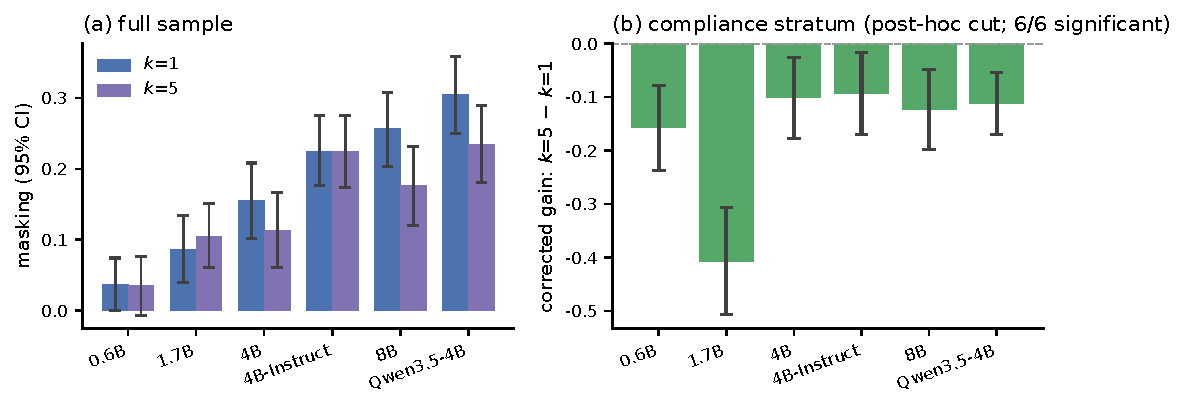
\includegraphics[width=\linewidth]{figures/fig5_kaxis.pdf}
\caption{The decision axis as an instance. (a) Full-sample masking at $k{=}1$ and $k{=}5$
(note the one reversal at 8B under $k{=}5$); (b) the paired compliance-stratum difference,
significant for 6/6 models, drawn with the same sign convention as $\Delta_{\text{strat}}$ in
Table~\ref{tab:bline} so that negative means $k{=}1$ is higher. We report the primary
criterion here and the weaker secondary ones in text.}
\label{fig:kaxis}
\end{figure}

% ============================================================================
\section{Design implications}
% ============================================================================
\begin{enumerate}\itemsep2pt
\item \textbf{Report a corrected gain, not only an apparent one.} The four-arm design costs
one extra arm pair; it converts an uninterpretable number into a bounded one.
\item \textbf{Make the plant credible but untrue.} Absurd plants are detected and rejected
by the model, which suppresses the measured compliance and biases the estimate. Our era
constraint moved the median plant distance from 69 to 7 years and removed a spurious
sign reversal.
\item \textbf{Do not infer memory from an oracle-accuracy drop.} That gate mixes unusable
evidence with the effect under study.
\item \textbf{When the effect is bounded away, report the bound, not a null result.}
The HotpotQA result is the most informative here: with an equivalence test it locates the
boundary instead of merely failing to detect an effect.
\end{enumerate}

% ============================================================================
\section{Limitations}
% ============================================================================
\begin{itemize}\itemsep2pt
\item \textbf{Borrowing rules are only established and comparable for numeric and date
answers.} We did test entity answers (\S\ref{sec:entity}) and attacked both of the biases that
would limit what that section can support: the entity pool is contaminated at a low rate by
numeric-form answers classified as names ($6.0\%$ of its $1{,}067$ items contain digits, and
$19$ items also appear in the numeric/date pool under a different answer spelling), and the
substituted-arm scorer is asymmetric (single canonical key versus the full answer list). We
recomputed the arm with an alias-aware rescoring and on the cleaned sub-pool; masking stays
negative in every variant, so the \emph{sign} of the entity result is not an artifact of either
bias---what the variants move is its depth, and for 8B whether the rule contrast is
distinguishable from zero (Table~\ref{tab:entity-robust}). Two residual gaps remain: plants
whose value is the same entity under a name that is \emph{not} in the target question's answer
list are unguarded, and a fully alias-aware scorer would need per-item human judgement of what
counts as the same entity. On the numeric/date line the trap is weaker because a value has
fewer accepted forms: $0.46\%$ of substitutions (two items per run) are no-ops, and removing
them moves every masking value by at most $0.003$ (\S\ref{sec:entity}, Table~\ref{tab:trap}).
\item \textbf{The audit covers a 20.2\% sample.} We do not extrapolate beyond the
corpus-level rate estimate, which we report as an implication rather than a measurement.
Treating the human audit ($22$ flagged items) and the verifier ($43$) as two captures of the
same defect population, a capture--recapture estimate puts the pre-fix corpus at
$\approx 24\%$ ($43\times22/9/446$; Chapman-corrected $22.5\%$). Applying the \emph{same}
estimator to the fixed corpus gives $\approx 26\%$ ($37\times18/6/432$; Chapman $23.6\%$), so
we \emph{cannot} claim that the fixes lowered the estimated residual rate---that estimate
rests on only six overlapping items, and its item-bootstrap interval is $[15\%,63\%]$. What
the fixes demonstrably did is remove the two defect classes we identified, which is why
dropping every audited item moves each of the $20$ masking values by at most $0.003$
(\S\ref{sec:validity}). Two caveats bound the rate itself: the verifier was run on the pre-fix
pool, so the fixed corpus is scored by transferring its flags rather than by a fresh pass, and
the recall figure rests on the $22$ human-judged items it found.
\item \textbf{Bottom-up construction quality is bounded by human effort.} Our LLM
pre-screen has $\approx$45\% recall and is not a substitute for auditing.
\item \textbf{Cross-generation evidence uses one model, and environments differ}
(transformers 4.51.3 vs 5.17.0); Qwen3.5-4B-Base is a vision-language architecture, so the
comparison is not modality-matched.
\item \textbf{The dense $k$ axis exists for one model on the final corpus.} For Qwen3-8B we have
the full $k\in\{1,3,5,10,20\}$ grid on the fixed corpus ($n{=}432$,
Table~\ref{tab:app-kaxis5}): every depth above $k{=}1$ has significantly \emph{smaller} masking
(paired $\Delta\mask$ from $-0.069$ to $-0.100$, all 95\% intervals excluding zero) while the
apparent gain is significantly \emph{larger} ($+0.046$ to $+0.051$), and at $k{=}10$ and $k{=}20$
the corrected gain is significantly lower than at $k{=}1$ ($-0.051$ and $-0.042$); the argmax
flips ($k{=}5$ on apparent, $k{=}1$ on corrected) in $0.854$ of resamples, above the $0.80$ bar,
though the pre-registered rule still returns ``do not change'' because the two competing
corrected-gain intervals overlap. This supersedes the $148$-item v0 pilot that previously
carried the axis. What is still missing is the other five models, for which only
$k\in\{1,5\}$ exists.
\item \textbf{The pool is deliberately enriched and is not representative.} We keep only
questions whose answer can be replaced under a type constraint, with a unique terminal
match. Answers of that shape---a single numeric or date token---are exactly the ones a model
is most likely to have memorised outright, so the levels reported here should be read as
values \emph{on this pool}, not as an estimate of masking for RAG over arbitrary factoid
questions. We have no measurement of masking on questions whose answers cannot be
type-substituted.
\item \textbf{Two relevance-oriented gates in the pipeline remain unresolved}
(the closed-book-collapse gate is ABANDON and the compliance gate REVISE under the frozen
thresholds); we treat them as limitations rather than evidence.
\item \textbf{Every number here was recomputed offline} with the frozen v3 scorer. One
earlier run stored its oracle fields under the previous (v2) scorer; we never quote those
stored values, and all comparisons are made under a single scorer.
\item \textbf{The B-line's closed-book and open-book arms do not depend on the
substitution}, so they are bit-identical between the two corpora---we use that as a
reproducibility check---except for a single TriviaQA item, where 4-bit CUDA inference is not
deterministic.
\item \textbf{All runs use 4-bit quantisation}, which we did not ablate: quantisation is
known to affect both recall of memorised facts and willingness to follow context, so the
absolute levels here should not be read as full-precision numbers. The contrast between
pools and between $k$ values is measured within a fixed quantisation scheme.
\item \textbf{Borrowed values can recur across questions}, so items are not strictly
independent. We check this rather than only disclosing it: resampling whole borrowed values
instead of questions moves every primary interval by at most $0.015$ and changes no
conclusion (Table~\ref{tab:cluster}).
\end{itemize}

% ============================================================================
\section{Conclusion}
% ============================================================================
Evaluating RAG by the gain over a closed-book baseline assumes the baseline is empty. We
measured what happens when it is not: on the retrieval line the apparent gain understates
the evidence's contribution by up to 31 accuracy points (the largest value comes from the
cross-generation model, which is not modality-matched), and at $k{=}1$ the shortfall grows
with scale. We then audited our own manipulation, found 24.4\% of it invalid, traced three root causes,
fixed two, and showed the effect survives---indeed strengthens. Finally we gave an exact
decomposition and used it to describe where the effect is absent: the effect appears only
where the question
is in the model's parametric memory, so on multi-hop questions it is bounded away from
effects above five points and is not removed by a stronger model, and on entity-type answers
an active, credible borrowing rule does not produce it either---while the audit of that rule
caught a trap (plants that were another name for the true answer) that would have made us
report the opposite. We hope the paper is read
less as a new RAG method than as a reason to change how RAG results are reported, and as a
worked example of auditing a controlled corpus before drawing conclusions from it.

\bibliographystyle{plainnat}
\bibliography{refs}

\appendix
% ============================================================================
%  Appendix A --- generated by rag_leak/make_appendix.py. Do not edit by hand.
%  Sources: rag_leak/out_*/metrics.json, fourarm.jsonl, out_sensitivity.json,
%           anno_defects_90.json, out_b8_audit_summary.json
%  NOTE: tables are deliberately NON-floating (captionof + center), because floating
%        them lets LaTeX drift a table past its own heading and leave the heading bare.
% ============================================================================
\section{Full numbers}
\label{app:full}

This appendix reports the numbers behind every figure and table in the main text. All of them are read directly from the per-question artifacts accompanying this paper.

\subsection{B-line: four arms, six models, both depths}
\begin{center}\small
\begin{minipage}{\linewidth}
\captionof{table}{TriviaQA B-line, final construction (v2), $n{=}432$ questions per cell, shared-corpus BM25 retrieval. Each row is one model at one depth; $a/b/c/d$ are the four arm accuracies and $\mask=(a-c)-(b-d)$. The interval is the paired-bootstrap interval for masking, so the ``10 of 12'' claim in the abstract can be checked row by row: only the 0.6B model's two intervals touch zero.}
\label{tab:app-bline}
\begin{tabular}{llrrrrr}
\toprule
Model & $k$ & $a$ & $b$ & $c$ & $d$ & \mask\ (95\% CI) \\
\midrule
Qwen3-0.6B & 1 & 0.102 & 0.421 & 0.009 & 0.366 & +0.037 [-0.000, +0.074] \\
Qwen3-0.6B & 5 & 0.102 & 0.435 & 0.009 & 0.377 & +0.035 [-0.007, +0.076] \\
\midrule
Qwen3-1.7B & 1 & 0.213 & 0.380 & 0.009 & 0.262 & +0.086 [+0.039, +0.134] \\
Qwen3-1.7B & 5 & 0.213 & 0.296 & 0.009 & 0.197 & +0.104 [+0.060, +0.150] \\
\midrule
Qwen3-4B & 1 & 0.382 & 0.604 & 0.012 & 0.389 & +0.155 [+0.102, +0.208] \\
Qwen3-4B & 5 & 0.382 & 0.634 & 0.012 & 0.377 & +0.113 [+0.060, +0.167] \\
\midrule
Qwen3-4B-Instruct & 1 & 0.363 & 0.484 & 0.007 & 0.352 & +0.225 [+0.176, +0.275] \\
Qwen3-4B-Instruct & 5 & 0.363 & 0.470 & 0.007 & 0.338 & +0.225 [+0.174, +0.275] \\
\midrule
Qwen3-8B & 1 & 0.472 & 0.556 & 0.007 & 0.347 & +0.257 [+0.204, +0.308] \\
Qwen3-8B & 5 & 0.472 & 0.606 & 0.007 & 0.317 & +0.176 [+0.120, +0.231] \\
\midrule
Qwen3.5-4B-Base & 1 & 0.558 & 0.694 & 0.021 & 0.463 & +0.306 [+0.250, +0.359] \\
Qwen3.5-4B-Base & 5 & 0.558 & 0.759 & 0.021 & 0.456 & +0.234 [+0.181, +0.289] \\
\bottomrule
\end{tabular}
\end{minipage}
\end{center}

\subsection{HotpotQA: four arms and the gate}
\begin{center}\small
\captionof{table}{HotpotQA C-line, final construction (v2), $n{=}393$, context budget 4096. The last column is the oracle-answerability gate of \S\ref{sec:gate3}: the drop in accuracy between the original and substituted gold evidence. The frozen thresholds are $\leq 3\%$ GO, $\leq 8\%$ REVISE, $>8\%$ ABANDON. The drop is an \emph{aggregate} difference, so a value of $0.0\%$ can arise from cancellation rather than from the substitution changing nothing: the two arms disagree item by item on Qwen3-0.6B (40/393 items), Qwen3-1.7B (33/393 items), Qwen3-8B (16/393 items), Qwen3-4B (16/393 items), Qwen3.5-4B-Base (18/393 items); for Qwen3-0.6B and Qwen3-4B these disagreements are exactly balanced, which is what makes the aggregate drop zero there.}
\label{tab:app-hotpot}
\begin{tabular}{lrrrrrr}
\toprule
Model & $a$ & $b$ & $c$ & $d$ & \mask & gate drop \\
\midrule
Qwen3-0.6B & 0.010 & 0.270 & 0.013 & 0.252 & -0.020 & 0.0\% \\
Qwen3-1.7B & 0.031 & 0.104 & 0.005 & 0.087 & +0.008 & 0.8\% \\
Qwen3-8B & 0.051 & 0.517 & 0.005 & 0.463 & -0.008 & 1.5\% \\
Qwen3-4B & 0.056 & 0.509 & 0.008 & 0.461 & +0.000 & 0.0\% \\
Qwen3.5-4B-Base & 0.056 & 0.529 & 0.015 & 0.473 & -0.015 & 2.5\% \\
\bottomrule
\end{tabular}
\end{center}

\subsection{Sensitivity of the compliance-stratum result to the cut}
\begin{center}\small
\captionof{table}{Paired $k{=}5$ minus $k{=}1$ difference in corrected gain under two nested definitions of the stratum. \emph{Broad} requires only that the planted value occurs in the retrieved context; \emph{strict} additionally requires that the model adopted it (the two stricter subsets we computed coincide exactly, so they are reported once). Signs are negative in all 12 cells; significance is confined to the strict cut.}
\label{tab:sens}
\begin{tabular}{lrrrr}
\toprule
 & \multicolumn{2}{c}{broad} & \multicolumn{2}{c}{strict} \\
\cmidrule(lr){2-3}\cmidrule(lr){4-5}
Model & $n$ & $\Delta$ (95\% CI) & $n$ & $\Delta$ (95\% CI) \\
\midrule
Qwen3-0.6B & 408 & +0.007 [-0.037, +0.054] & 190 & -0.158 [-0.237, -0.079] \\
Qwen3-1.7B & 408 & -0.066 [-0.115, -0.017] & 140 & -0.407 [-0.507, -0.307] \\
Qwen3-4B & 408 & -0.012 [-0.054, +0.029] & 198 & -0.101 [-0.177, -0.025] \\
Qwen3-4B-Instruct & 408 & -0.015 [-0.054, +0.025] & 183 & -0.093 [-0.169, -0.016] \\
Qwen3-8B & 408 & -0.029 [-0.066, +0.010] & 186 & -0.124 [-0.199, -0.048] \\
Qwen3.5-4B-Base & 408 & -0.007 [-0.049, +0.037] & 241 & -0.112 [-0.170, -0.054] \\
\bottomrule
\end{tabular}
\end{center}

\noindent Leave-one-model-out on the pooled strict stratum (1138 item-level differences): dropping any single model leaves the pooled $\Delta$ between $-0.12$ and $-0.16$, with every interval excluding zero (Table~\ref{tab:app-loo}).

\begin{center}\small
\captionof{table}{Pooled strict-stratum difference with each model dropped in turn.}
\label{tab:app-loo}
\begin{tabular}{lrrr}
\toprule
Dropped & $n$ & $\Delta$ & 95\% CI \\
\midrule
none (all models) & 1138 & -0.153 & [-0.186, -0.122] \\
drop Qwen3-0.6B & 948 & -0.152 & [-0.187, -0.119] \\
drop Qwen3-1.7B & 998 & -0.117 & [-0.152, -0.085] \\
drop Qwen3-4B & 940 & -0.164 & [-0.197, -0.130] \\
drop Qwen3-4B-Instruct & 955 & -0.164 & [-0.199, -0.131] \\
drop Qwen3-8B & 952 & -0.159 & [-0.193, -0.124] \\
drop Qwen3.5-4B-Base & 897 & -0.164 & [-0.200, -0.127] \\
\bottomrule
\end{tabular}
\end{center}

\subsection{Clustered bootstrap over borrowed values}
\begin{center}\small
\captionof{table}{Primary stratum contrast with two resampling schemes. The same planted value can recur across items, so we also resample whole values (clusters) rather than questions. No conclusion changes; the largest interval movement is $0.015$.}
\label{tab:cluster}
\begin{tabular}{lrrrrr}
\toprule
Model & items & clusters & $\Delta$ & CI (by item) & CI (by value) \\
\midrule
Qwen3-0.6B & 190 & 108 & -0.158 & [-0.237, -0.079] & [-0.239, -0.079] \\
Qwen3-1.7B & 140 & 87 & -0.407 & [-0.507, -0.307] & [-0.507, -0.309] \\
Qwen3-4B & 198 & 104 & -0.101 & [-0.177, -0.025] & [-0.183, -0.020] \\
Qwen3-4B-Instruct & 183 & 96 & -0.093 & [-0.169, -0.016] & [-0.167, -0.022] \\
Qwen3-8B & 186 & 94 & -0.124 & [-0.199, -0.048] & [-0.214, -0.035] \\
Qwen3.5-4B-Base & 241 & 116 & -0.112 & [-0.170, -0.054] & [-0.175, -0.047] \\
\bottomrule
\end{tabular}
\end{center}

\subsection{The audited defects, item by item}
\begin{center}\small
\begin{minipage}{\linewidth}
\captionof{table}{All 22 items judged invalid in the 90-item audit. Indices are the audit's own; ``flagged'' records which annotator(s) caught the item, so the two both-missed cases are visible. The four classes map onto the three root causes of \S\ref{sec:validity} as described there.}
\label{tab:app-audit}
\begin{tabular}{rlrl}
\toprule
\# & item & class & flagged \\
\midrule
3 & \texttt{trivia-106} & wrong position & missed by both \\
4 & \texttt{trivia-110} & wrong position & both \\
12 & \texttt{trivia-147} & malformed value & one \\
15 & \texttt{trivia-160} & malformed value & both \\
17 & \texttt{trivia-17} & wrong position & both \\
23 & \texttt{trivia-198} & malformed value & one \\
26 & \texttt{trivia-21} & wrong position & both \\
32 & \texttt{trivia-238} & wrong position & both \\
37 & \texttt{trivia-260} & wrong position & both \\
45 & \texttt{trivia-297} & new = true answer & both \\
49 & \texttt{trivia-313} & wrong position & both \\
50 & \texttt{trivia-318} & wrong position & one \\
51 & \texttt{trivia-322} & wrong position & both \\
53 & \texttt{trivia-331} & wrong position & both \\
54 & \texttt{trivia-336} & wrong position & both \\
55 & \texttt{trivia-340} & wrong position & both \\
67 & \texttt{trivia-395} & wrong position & missed by both \\
68 & \texttt{trivia-4} & wrong position & both \\
71 & \texttt{trivia-411} & wrong position & one \\
76 & \texttt{trivia-435} & wrong position & both \\
85 & \texttt{trivia-72} & wrong position & both \\
88 & \texttt{trivia-86} & self-contradictory & one \\
\bottomrule
\end{tabular}
\end{minipage}
\end{center}

\subsection{The LLM pre-screen is a weak filter}
On the 90 audited items the span-verification probe recovers 10 of the 22 defects while flagging 3 of the 68 usable items (Table~\ref{tab:app-prescreen}). Applied to the whole 446-item list it flags 43, at a rate that matches between the audited sample (11.1\%) and the rest (9.3\%).

\begin{center}\small
\captionof{table}{LLM span-verification probe against the human audit ($n{=}90$).}
\label{tab:app-prescreen}
\begin{tabular}{lrr}
\toprule
 & flagged invalid & judged valid \\
\midrule
human: invalid & 10 & 12 \\
human: valid & 3 & 65 \\
\bottomrule
\end{tabular}
\end{center}

\subsection{Cleaning ablations}
\begin{center}\small
\begin{minipage}{\linewidth}
\captionof{table}{Recomputing the decision-axis contrast after removing flagged items. Every cell keeps its sign; the effect is diluted by the bad items rather than created by them. Computed on the pre-fix (v0) corpus, which is why the levels differ from the v2 numbers in the main text.}
\label{tab:app-cleaning-v0}
\begin{tabular}{llrrrr}
\toprule
Model & scope & $n$ & \mask($k{=}1$) & \mask($k{=}5$) & $\Delta$masking (95\% CI) \\
\midrule
Qwen3-8B & all items & 446 & 0.184 & 0.090 & -0.094 [-0.135, -0.054] \\
Qwen3-8B & audited sample & 90 & 0.189 & 0.111 & -0.078 [-0.167, +0.011] \\
Qwen3-8B & after removing flagged & 68 & 0.235 & 0.176 & -0.059 [-0.162, +0.044] \\
Qwen3.5-4B-Base & all items & 446 & 0.244 & 0.143 & -0.101 [-0.143, -0.058] \\
Qwen3.5-4B-Base & audited sample & 90 & 0.300 & 0.222 & -0.078 [-0.167, +0.011] \\
Qwen3.5-4B-Base & after removing flagged & 68 & 0.382 & 0.294 & -0.088 [-0.191, +0.015] \\
Qwen3-0.6B & all items & 446 & 0.027 & -0.007 & -0.034 [-0.081, +0.013] \\
Qwen3-0.6B & audited sample & 90 & -0.022 & -0.067 & -0.044 [-0.156, +0.056] \\
Qwen3-0.6B & after removing flagged & 68 & -0.088 & -0.103 & -0.015 [-0.147, +0.118] \\
Qwen3-1.7B & all items & 446 & 0.078 & 0.083 & +0.004 [-0.040, +0.049] \\
Qwen3-1.7B & audited sample & 90 & -0.022 & 0.089 & +0.111 [+0.000, +0.222] \\
Qwen3-1.7B & after removing flagged & 68 & -0.029 & 0.088 & +0.118 [-0.015, +0.250] \\
Qwen3-4B & all items & 446 & 0.078 & -0.000 & -0.078 [-0.126, -0.034] \\
Qwen3-4B & audited sample & 90 & 0.056 & -0.000 & -0.056 [-0.156, +0.044] \\
Qwen3-4B & after removing flagged & 68 & 0.044 & -0.044 & -0.088 [-0.206, +0.044] \\
Qwen3-4B-Instruct & all items & 446 & 0.150 & 0.126 & -0.025 [-0.065, +0.016] \\
Qwen3-4B-Instruct & audited sample & 90 & 0.211 & 0.200 & -0.011 [-0.111, +0.089] \\
Qwen3-4B-Instruct & after removing flagged & 68 & 0.265 & 0.250 & -0.015 [-0.132, +0.103] \\
\bottomrule
\end{tabular}
\end{minipage}
\end{center}

\subsection{The oracle-answerability gate on TriviaQA}
\begin{center}\small
\captionof{table}{TriviaQA C-line, final construction (v2), $n{=}432$. The gate never turns GO here, which is the point of \S\ref{sec:gate3}: on our reading the residual drop is the treatment effect rather than a defect in the evidence.}
\label{tab:app-trivia-gate}
\begin{tabular}{lrrr}
\toprule
Model & oracle (original) & oracle (substituted) & drop \\
\midrule
Qwen3-0.6B & 0.491 & 0.444 & 4.6\% \\
Qwen3-1.7B & 0.428 & 0.329 & 10.0\% \\
Qwen3-4B & 0.681 & 0.465 & 21.5\% \\
Qwen3-4B-Instruct & 0.569 & 0.431 & 13.9\% \\
Qwen3-8B & 0.664 & 0.435 & 22.9\% \\
\bottomrule
\end{tabular}
\end{center}

\subsection{Cleaning the fixed corpus, every model}
\begin{center}\small
\begin{minipage}{\linewidth}
\captionof{table}{Every run recomputed with the audited items removed: the union of the 22 human-judged invalid and the 43 model-flagged items is 56 distinct items, of which \textbf{49 lie in the fixed (v2) corpus} and 7 were already dropped by the fixes recorded in \S\ref{sec:validity}; the HotpotQA rows lose none, because the audit was drawn from the TriviaQA pool. All 20 cells keep their sign and their significance; masking moves slightly upward, i.e.\ the invalid items dilute the effect rather than create it. The unchanged HotpotQA rows are therefore not evidence of robustness.}
\label{tab:app-cleaning}
\begin{tabular}{lrrrrr}
\toprule
Run & $n$ & $n$ (cleaned) & \mask & \mask\ (cleaned) & sign/significance \\
\midrule
B:Qwen3-0.6B k1 & 432 & 383 & +0.037 & +0.031 & unchanged \\
B:Qwen3-0.6B k5 & 432 & 383 & +0.035 & +0.039 & unchanged \\
B:Qwen3-1.7B k1 & 432 & 383 & +0.086 & +0.089 & unchanged \\
B:Qwen3-1.7B k5 & 432 & 383 & +0.104 & +0.099 & unchanged \\
B:Qwen3-4B-Instruct k1 & 432 & 383 & +0.225 & +0.240 & unchanged \\
B:Qwen3-4B-Instruct k5 & 432 & 383 & +0.225 & +0.230 & unchanged \\
B:Qwen3-4B k1 & 432 & 383 & +0.155 & +0.154 & unchanged \\
B:Qwen3-4B k5 & 432 & 383 & +0.113 & +0.112 & unchanged \\
B:Qwen3-8B k1 & 432 & 383 & +0.257 & +0.277 & unchanged \\
B:Qwen3-8B k5 & 432 & 383 & +0.176 & +0.191 & unchanged \\
B:Qwen3.5-4B-Base k1 & 432 & 383 & +0.306 & +0.337 & unchanged \\
B:Qwen3.5-4B-Base k5 & 432 & 383 & +0.234 & +0.264 & unchanged \\
C:Qwen3-0.6B & 432 & 383 & +0.032 & +0.037 & unchanged \\
C:Qwen3-1.7B & 432 & 383 & +0.095 & +0.099 & unchanged \\
C:Qwen3-4B & 432 & 383 & +0.134 & +0.144 & unchanged \\
C:Qwen3-4B-Instruct & 432 & 383 & +0.213 & +0.225 & unchanged \\
C:Qwen3-8B & 432 & 383 & +0.231 & +0.264 & unchanged \\
H:Qwen3-4B & 393 & 393 & +0.000 & +0.000 & unchanged \\
H:Qwen3-8B & 393 & 393 & -0.008 & -0.008 & unchanged \\
H:Qwen3.5-4B-Base & 393 & 393 & -0.015 & -0.015 & unchanged \\
\bottomrule
\end{tabular}
\end{minipage}
\end{center}

\subsection{The identity, seen item by item}
\begin{center}\small
\begin{minipage}{\linewidth}
\captionof{table}{Each run's items split by whether the model answered correctly closed-book. Masking is positive on the questions the model already knew and slightly negative elsewhere. The gap between strata is bounded near $1$ by construction, because $a$ differs by exactly $1$ between them; we report this as an illustration of the identity, not as independent evidence.}
\label{tab:app-conditional}
\begin{tabular}{lrrrr}
\toprule
Run & $n$ ($a{=}1$) & \mask\ ($a{=}1$) & $n$ ($a{=}0$) & \mask\ ($a{=}0$) \\
\midrule
B:Qwen3-0.6B k1 & 44 & +0.545 & 388 & -0.021 \\
B:Qwen3-0.6B k5 & 44 & +0.636 & 388 & -0.034 \\
B:Qwen3-1.7B k1 & 92 & +0.696 & 340 & -0.079 \\
B:Qwen3-1.7B k5 & 92 & +0.696 & 340 & -0.056 \\
B:Qwen3-4B-Instruct k1 & 157 & +0.726 & 275 & -0.062 \\
B:Qwen3-4B-Instruct k5 & 157 & +0.732 & 275 & -0.065 \\
B:Qwen3-4B k1 & 165 & +0.624 & 267 & -0.135 \\
B:Qwen3-4B k5 & 165 & +0.503 & 267 & -0.127 \\
B:Qwen3-8B k1 & 204 & +0.647 & 228 & -0.092 \\
B:Qwen3-8B k5 & 204 & +0.549 & 228 & -0.158 \\
B:Qwen3.5-4B-Base k1 & 241 & +0.651 & 191 & -0.131 \\
B:Qwen3.5-4B-Base k5 & 241 & +0.552 & 191 & -0.168 \\
C:Qwen3-0.6B & 44 & +0.523 & 388 & -0.023 \\
C:Qwen3-1.7B & 92 & +0.761 & 340 & -0.085 \\
C:Qwen3-4B & 165 & +0.564 & 267 & -0.131 \\
C:Qwen3-4B-Instruct & 157 & +0.713 & 275 & -0.073 \\
C:Qwen3-8B & 204 & +0.637 & 228 & -0.132 \\
H:Qwen3-4B & 22 & +0.773 & 371 & -0.046 \\
H:Qwen3-8B & 20 & +0.950 & 373 & -0.059 \\
H:Qwen3.5-4B-Base & 22 & +0.727 & 371 & -0.059 \\
\bottomrule
\end{tabular}
\end{minipage}
\end{center}

\subsection{B-line $k$ axis on the final corpus (five depths)}
\begin{center}\small
\captionof{table}{B-line $k$ axis for Qwen3-8B on the fixed corpus ($n{=}432$). The corpus is identical across depths (closed-book arms are bit-identical item by item), so the only difference is how much context retrieval supplies. $\Delta$ is paired against $k{=}1$ with an item bootstrap; the interval for $\Delta\mask$ excludes zero at every depth above $k{=}1$. The last two columns are from the five-way argmax resampling of \S\ref{sec:decision}.}
\label{tab:app-kaxis5}
\begin{tabular}{rrrrrrrr}
\toprule
$k$ & $a$ & apparent & corrected & \mask & $\Delta$\mask\ (95\% CI) & $\Delta$apparent & $\Delta$corrected \\
\midrule
1 & 0.472 & +0.083 & +0.340 & +0.257 & --- & --- & --- \\
3 & 0.472 & +0.130 & +0.317 & +0.188 & $-0.069$ $[-0.109,-0.030]$ & +0.046 & -0.023 \\
5 & 0.472 & +0.134 & +0.310 & +0.176 & $-0.081$ $[-0.125,-0.039]$ & +0.051 & -0.030 \\
10 & 0.472 & +0.132 & +0.289 & +0.157 & $-0.100$ $[-0.144,-0.056]$ & +0.049 & -0.051 \\
20 & 0.472 & +0.132 & +0.299 & +0.167 & $-0.090$ $[-0.134,-0.046]$ & +0.049 & -0.042 \\
\bottomrule
\end{tabular}
\end{center}
Five-way argmax: apparent prefers $k=5$, corrected prefers $k=1$; the argmax changes in $0.854$ of resamples (threshold $0.80$), but the pre-registered rule still returns ``do not change'' because the two competing corrected-gain intervals overlap.

\subsection{Disclosures}
\begin{itemize}\itemsep1pt
\item Agreement is reported under both readings ($\kappa{=}0.82$ and $0.78$); four items were decided only after the annotators conferred, which compromises their independence.
\item The cross-generation check compares models run under two library stacks (transformers 4.51.3 and 5.17.0), and Qwen3.5-4B-Base is a vision-language architecture, so that comparison is not modality-matched.
\item The oracle-answerability gate still returns ABANDON on TriviaQA; our reading of the residual as genuine memory resistance is an interpretation, not a measurement.
\item Three corpus versions exist (v0, v1, v2); every headline number is from v2, and the cross-generation contrast in \S\ref{sec:precond} is drawn from v2 artifacts.
\item The audit covers 20.2\% of the construction list; we do not extrapolate beyond the corpus-level rate estimate.
\item The compliance stratum is a post-hoc cut; see the sensitivity analysis above.
\item On the pre-fix corpus 1.7B showed more masking than 4B; on the fixed corpus that reversal is gone and the step moves by $+0.065$ (95\% CI $[+0.019,+0.111]$). Neither corpus shows the reversal individually, so we report the movement, not a reversal.
\item All runs use 4-bit quantisation, which we did not ablate.
\item Borrowed values can recur across items; the clustered bootstrap above addresses this and changes no conclusion.
\item One pipeline run stored its oracle fields under an earlier scorer; every number here was recomputed offline with the frozen v3 scorer instead.
\item Code, corpora and audit materials: \url{https://anonymous.4open.science/r/ragmask-9c41d7b/}.
\item HotpotQA contains no single-hop sub-population, so the multi-hop result cannot be explained by a subset of single-hop questions.
\item Environment and seeds, for reproduction: a single NVIDIA RTX 4060 Laptop GPU with 8\,GB, 4-bit weights via bitsandbytes 0.45.5, PyTorch 2.5.1+cu121 (CUDA 12.1), transformers 4.51.3 for the Qwen3 family and 5.17.0 for Qwen3.5-4B-Base. Question sampling from each pool and every bootstrap use the same fixed seed, 20260903 ($B{=}10{,}000$ resamples); the sampling seed makes each compared pair of conditions see an identical item set, which we verify rather than assume.
\item The entity experiment (\S\ref{sec:entity}) additionally discloses that its closed-book arm is scored against a single canonical key while the original-answer arms use the full answer list, and that this asymmetry biases the entity-line masking downward---i.e.\ in the direction of the null reported there.
\end{itemize}


\end{document}
